\documentclass[letterpaper,twocolumn,10pt]{article}

\usepackage[utf8]{inputenc}
\usepackage{usenix}
\usepackage{tikz}
\usepackage{xcolor} % For colourful links.
\usepackage[backend=biber,backref=true,maxnames=20,urldate=long]{biblatex}
\usepackage{hyperref} % For clickable links.
\hypersetup{draft}
\usepackage[l2tabu, orthodox]{nag}
\usepackage{subcaption}
\usepackage{booktabs}
\usepackage{enumitem} % For custom symbols in enumerations.
\usepackage{wasysym}  % For \Square and \Circle.
\usepackage[english]{babel}
\usepackage{csquotes}
\usepackage[nameinlink]{cleveref}
\usepackage{fontawesome} % For the link icon in the bibliography.
\usepackage{balance}

\usepackage[T1]{fontenc}
\usepackage[scaled=0.8]{beramono}
\usepackage[scaled=0.8]{berasans}

\urlstyle{rm}

\addbibresource{paper.bib}

\definecolor{darkblue}{rgb}{0.1,0.1,0.4}

% Use a link icon instead of BibLaTeX's "URL" string.
\DeclareFieldFormat{url}{{\scriptsize \faExternalLink}~\url{#1}}

\usetikzlibrary{positioning}

\newcommand{\ie}{i.e.}
\newcommand{\eg}{e.g.}
\newcommand{\ea}{et al.}
\newcommand{\first}{(\textit{i})}
\newcommand{\second}{(\textit{ii})}
\newcommand{\third}{(\textit{iii})}
\newcommand{\fourth}{(\textit{iv})}
\newcommand{\fifth}{(\textit{v})}
\newcommand{\mc}[1]{\textcolor{blue}{\noindent[MC: #1]}}
\newcommand{\adz}[1]{\textcolor{red}{\noindent[ADZ: #1]}}
\newcommand{\annie}[1]{\textcolor{orange}{\noindent#1}}

\hypersetup{
	pdftitle={How do Tor users interact with onion services?},
	pdfauthor={Philipp Winter, Anne Edmundson, Laura M. Roberts, Marshini Chetty, and Nick Feamster},
	pdfkeywords={Tor, usability, anonymity, usable security},
	colorlinks=true,
	urlcolor=darkblue,
	linkcolor=darkblue,
	citecolor=darkblue
}

\renewcommand*{\bibfont}{\small}

\begin{document}

% Don't want date printed
\date{}

\title{
    {\Large \textbf{How Do Tor Users Interact With Onion Services?}}
}

\author{
	{\rm \phantom{ZZZZ}Philipp Winter\phantom{ZZZZ}} \\
	Princeton University
	\and
	{\rm \phantom{ZZZZ}Anne Edmundson\phantom{ZZZZ}} \\
	Princeton University
	\and
	{\rm \phantom{ZZZ}Laura M. Roberts\phantom{ZZZ}} \\
	Princeton University
	\and
	{\rm Agnieszka Dutkowska-Żuk} \\
	Independent
	\and
	{\rm \phantom{ZZZZ}Marshini Chetty\phantom{ZZZZ}} \\
	Princeton University
	\and
	{\rm \phantom{ZZZZ}Nick Feamster\phantom{ZZZZ}} \\
	Princeton University
}

\maketitle

% Use the following at camera-ready time to suppress page numbers.
% Comment it out when you first submit the paper for review.
\thispagestyle{empty}

\subsection*{Abstract}
% Problem statement.
Onion services are anonymous TCP services that are exposed over the Tor network.
Compared to conventional Internet services, onion services are barely indexed by
search engines; private by default; and employ long, self-authenticating domain
names.  Our understanding of how users handle these idiosyncrasies is anecdotal.
% What we are doing.
In this work we fill this gap by studying how people perceive, understand, and
use onion services.  To that end we explored the problem space by conducting
seventeen semi-structured interviews.  Having gained preliminary insight, we
then solicited answers to concrete questions by administering an online survey
that attracted 828 responses.  Our findings show that \first~onion service
discovery is met with dissatisfaction, but could be greatly improved with an
opt-in publishing mechanism; \second~users handle the non-memorable domain
format by employing diverse makeshift solutions, some of which Tor Browser could
provide; and \third~some users misunderstand the technology behind onion
services which may facilitate phishing attacks.
% Why our work matters.
Our work allows The Tor Project to focus its efforts on the most pressing
usability issues and to address common misconceptions by improving its
documentation, improving both security and usability in the process.


\section{Introduction}
\label{sec:introduction}
The Tor Project's onion services provide what may be the
most popular way of running an anonymous \textsc{tcp} service. Typically, online anonymity implies \emph{client} anonymity
such as the use of a \textsc{virtual private network} to disguise one's \textsc{ip} address.  However, Tor onion services employ a lesser-known use case of anonymity, that is \emph{server} anonymity which allows a web service to
disguise its \textsc{ip} address.  Service operators have good reasons to employ
server anonymity; be it to escape harassment, speak out against power, or voice
dissenting opinions.  \footnote{Onion
services were originally called ``hidden services'' but were recently renamed to
reflect the fact that onion services provide more than just ``hiding'' a
service~\cite{Johnson2015a}---most importantly end-to-end security and
self-authenticating names.}

Originally deployed in 2004, onion services have grown substantially over the
last years, both in the number of servers and users.  As of February 2018, The
Tor Project's statistics count more than 60,000 onion services each day,
relaying an aggregate of 1 Gbps of network traffic.  Not all of these services
host web sites; use cases such as metadata-free instant
messaging~\cite{ricochet} and file sharing~\cite{onionshare} have emerged as
well.  The Tor Project currently does not have data on the number of onion
service users but Facebook reported in 2016 that more than one million users
logged into their onion service over a one-month period~\cite{facebook-users}.

Onion services differ from conventional web services in several aspects;
\first~they can only be accessed over the Tor network; \second~onion domains are
hashes over their public key, rendering them hard to remember; \third~network
latency is noticeable because of the additional hops in between client and the
onion service; and \fourth~onion services are private by default, requiring
manual dissemination.  To date, our understanding of how users deal with these
idiosyncrasies is anecdotal.  We fill this gap by studying how Tor users
interact with onion services.

However, onion services do not exist in a vacuum.
They are tightly coupled to their
surrounding software ecosystem---most importantly, the Tor Browser---which is why an
isolated study of onion services without accounting for Tor is bound to miss crucial context.  Therefore, we set out to understand users'
mental models of onion services \emph{and} the Tor network where applicable, and we study 
how they use and manage onion services, the challenges and benefits of using onion services, and how they adapt their workflow to deal with onion services.

To that end, we employ a mixed-methods approach. First, we conducted exploratory interviews with Tor and onion service users to guide the design of an online survey. We then conducted a large scale online survey that featured an array of questions on Tor Browser, onion service usage and operation, onion site
phishing, and users' general expectations of privacy. Finally, we conducted follow up interviews to flesh out the topics uncovered in the exploratory interviews and the survey to allow us a deeper dive into the themes of interest.

Our findings include that \first~many Tor users misunderstand technical aspects
of onion services such as the nature of the domain format, rendering these users
more vulnerable to phishing attacks; \second~users handle the pseudo-random
onion domain format differently, but mostly by bookmarking them; and \third~the
way people discover onion services is provisional and in need of technical
enhancements to ease the process.

At the time of this writing, The Tor Project is testing the next generation of
onion services intended to fix security issues and upgrade to faster and
future-proof cryptography.  Our results can inform this process.
Finally, because some of our findings touch on general aspects of privacy and
anonymity, we believe that privacy engineers beyond The Tor Project can benefit
from our findings.  In summary, we make the following contributions:

\begin{itemize}
    \item We interviewed seventeen Tor users of diverse backgrounds to
        understand their issues, assumptions, and expectations related to the
        Tor network.  Using qualitative data coding, we identified and present
        themes and anecdotes that underlay our interview data.

    \item We administered an online survey for Tor users, gathering 527 full
        responses.  Our survey focused on the most salient issues around onion
        services, \ie, the domain format, onion service discovery, and phishing
        attacks.

    \item Drawing on our two datasets, we identify key issues that impede the
        adoption of onion services and propose ways forward, \eg, an opt-in
        publishing mechanism for onion services, and a Tor Browser extension
        that allows its users to securely bookmark onion domains without
        exposing a browsing trail.
\end{itemize}

The rest of this paper is structured as follows.  We begin by discussing related
work in \Cref{sec:related-work}, followed by background on onion services in
\Cref{sec:background}.  \Cref{sec:method} then presents the methods we used for
our interviews and online survey, followed by \Cref{sec:results} which discusses
our findings from both data sources.  Finally, we discuss our work in
\Cref{sec:discussion} and conclude in \Cref{sec:conclusion}.


\section{Related Work}
\label{sec:related-work}

The usability of Tor Browser has seen numerous substantial changes since its
creation in 2003~\cite{Syverson2005a}; from a manually-installed Tor ``button,''
to the Tor Browser Bundle, to the currently-used Tor Browser.  Installation has
not always been as easy as today, which prompted Clark, van Oorschot, and Adams
to use cognitive walkthroughs to study how users install, configure, and run
Tor Browser~\cite{Clark2007a}.  The authors uncovered usability hurdles such as
jargon-laden documentation, confusing menus, and insufficient visual feedback.
As of February 2018, the study is ten years old---Tor Browser has since seen
radical changes.

Much more recently, in 2014, Norcie \ea\ identified stop-points in the
installation and use of the Tor Browser Bundle~\cite{Norcie2014a}.\footnote{The
Tor Browser Bundle was later rebranded and is now known as Tor Browser.}  These
stop-points represent places in a user interface that require action but are met
instead with confusion by users.  Having identified these stop-points, the
authors then issued interface design recommendations and subsequently tested
these recommendations in a user study.

Inspired by Tor Browser's use as anti-censorship system, Fifield \ea\ published
a design to study its usability as a censorship circumvention
tool~\cite{Fifield2015a}.  By drawing on both qualitative and quantitative
methods, the authors plan to recruit hundreds of users to study how they use Tor
Browser's configuration wizard in an adversarial setting.  Lee
\ea~\cite{Lee2017a} studied the usability of Tor Launcher, the graphical
configuration tool that allows users to configure Tor Browser.  Their findings
paint a bleak picture: 79\% of users' connection attempts in a simulated
censored environment failed.  However, the researchers showed that their
proposed interface improvements resulted in less difficulties for users.

Forte \ea\ studied the privacy practices of contributors to open collaboration
projects~\cite{Forte2017a}.  The authors interviewed 23 contributors to The Tor
Project and Wikipedia to learn about how privacy concerns affect their
contribution practices.  The study found that contributors worry about an array
of threats including surveillance, violence, harassment, and loss of
opportunity.

Most recently in 2017, Gallagher \ea\ conducted a series of semi-structured
interviews to understand both why people use Tor Browser and how they understand
the technology~\cite{Gallagher2017a}.  The authors found that experts tend to
have a network-centric view of the Tor network and tend to use it frequently
while non-experts have a goal-oriented view and see Tor Browser as a black box
that provides a service.  Our own work supports these findings.  Consequently,
non-experts do not use Tor Browser if they do not need its service.
Furthermore, non-experts tend to consider a single threat while the threat model
of experts contains multiple actors.

Several research efforts sought to alleviate the handling of randomly-generated
domain names.  Sai and Fink proposed a mnemonic system that maps 80-bit onion
domains to sentences~\cite{Sai2012a}.  Their work is inspired by mnemonicode, a
method to map binary data to words~\cite{mnemonicode}.  Victors \ea\ proposed a
more radical approach by designing the Onion Name System~\cite{Victors2017a}
which allows users to reference an onion service by a meaningful and
globally-unique identifier.  Kadianakis \ea\ designed a modular name system
\textsc{api} that allows Tor clients to configure name systems (\eg,
\textsc{gns}~\cite{Schanzenbach2012a} or OnioNS~\cite{Victors2017a}) on a
per-domain basis~\cite{Kadianakis2016a}.  Kadianakis summarized the current
state of research on onion service naming systems in a blog
post~\cite{Kadianakis2017a}.

We improve on the existing body of work by studying unanswered questions about
the use of Tor Browser and---the focus of this paper---how users interact with
onion services.  We believe that some of our findings generalize to other
systems, \eg, Freenet~\cite{Freenet} and Bitcoin~\cite{Nakamoto2008a} also
employ self-authenticating names---Freenet in its file naming scheme and Bitcoin
in its addressing scheme.


\section{Background}
\label{sec:background}

Onion services are TCP services that are only accessible over the Tor network.
While conventional Internet services are contacted over their IP address, onion
services are contacted over their onion domain, which is resolved and routed
inside the Tor network.  Due to onion services being hosted in the Tor network,
network traffic traverses six Tor relays (see Figure~\ref{fig:onion-service})
before it reaches the onion service.  The resulting increase in latency is the
cost of the anonymity that onion services provide.

\begin{figure*}[ht]
\centering
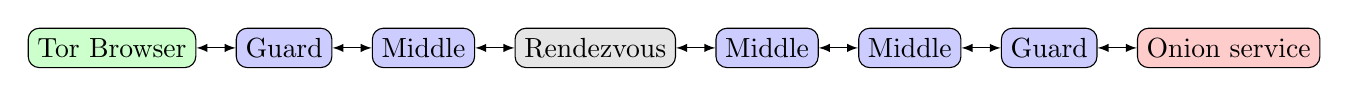
\begin{tikzpicture}[node distance=0.5cm]
\tikzset{>=latex}

\tikzstyle{block} = [rectangle, draw, rounded corners, text centered,
                     minimum height=0.5cm]

\node[block,fill=green!20]             (TB)  {Tor Browser};
\node[block,fill=blue!20,right=of TB]  (GR1) {Guard};
\node[block,fill=blue!20,right=of GR1] (MR1) {Middle};
\node[block,fill=gray!20,right=of MR1] (R)   {Rendezvous};
\node[block,fill=blue!20,right=of R]   (MR2) {Middle};
\node[block,fill=blue!20,right=of MR2] (MR3) {Middle};
\node[block,fill=blue!20,right=of MR3] (GR2) {Guard};
\node[block,fill=red!20,right=of GR2]  (OS)  {Onion service};

\draw[<->] (TB.east)  -- (GR1.west);
\draw[<->] (GR1.east) -- (MR1.west);
\draw[<->] (MR1.east) -- (R.west);
\draw[<->] (R.east)   -- (MR2.west);
\draw[<->] (MR2.east) -- (MR3.west);
\draw[<->] (MR3.east) -- (GR2.west);
\draw[<->] (GR2.east) -- (OS.west);

\end{tikzpicture}
\caption{When a user connects to an onion service, there are six relays in
between her Tor Browser (on the left) and the onion service (on the right).}
\label{fig:onion-service}
\end{figure*}

To create an onion domain, a Tor client first generates an RSA key pair.  It
then computes the SHA-1 hash over the RSA public key, truncates it to 80 bits,
and encodes these 80 bits in Base32, resulting in sixteen characters, \eg,
\texttt{expyuzz4wqqyqhjn}.  Due to the domain being a function of the public
key, onion domains are self-authenticating, meaning that as long as a client has
the correct domain, it knows what public key to expect.  The downside is that
sixteen random characters are impractical to remember.  However, onion domains
can be made at least partially meaningful by repeatedly creating RSA keys until
the resulting domain contains a desired string.  These domains are referred to
as \emph{vanity onion domains}.  The longer the desired string, the more time it
takes to find a matching key pair.  In practice, onion service operators use
tools such as scallion~\cite{scallion} that parallelize the search for suitable
keys to speed up the process.  Vanity domains are used by several organizations
such as Facebook (\url{facebookcorewwwi.onion}), ProPublica
(\url{propub3r6espa33w.onion}), and the New York Times
(\url{nytimes3xbfgragh.onion}).

Onion services are private by default.  Once an onion service is created, it is
up to its operator to announce it to the public, \eg, by adding it to onion site
search engines such as Ahmia.\footnote{The search engine is available online at
\url{https://ahmia.fi}.}  The lack of a go-to service such as Google for
onion service discovery means that the community has devised various ways to
publish onion services; most importantly an array of search engines and curated
lists.


\section{Method}
\label{sec:method}

We will now elaborate on how we designed our interviews
(\Cref{sec:interviews}) and our online survey
(\Cref{sec:online-survey}).  For both we will discuss participant
recruitment, how we structured the interview or survey process, and research
ethics.

\subsection{Interviews}
\label{sec:interviews}

We developed a question set that served as the basis for each
interview.\footnote{The question set is available online at
\url{https://nymity.ch/onion-services/pdf/interview-checklist.pdf}.}  The
semi-structured nature of our interviews allowed us to deviate from this
question set, \eg, by asking follow-up questions.  We began by asking
demographic information (gender, age range, occupation, country of residence,
and level of education), followed by information about online behavior, and
finally questions specific to Tor Browser and onion services.

\subsubsection{Procedure}

Princeton University's institutional review board (\textsc{irb}) deemed our
study exempt from further review.\footnote{Our \textsc{irb} protocol number is
8251.}  We conducted thirteen interviews in person and four interviews remotely;
over Skype, Signal, WhatsApp, and Jitsi---depending on what our interviewees
felt the most comfortable with.  For in-person interviews we asked our
interviewees to sign a consent form.  This was not practical for remote
interviews, so we sent the consent form in advance, over email, and after
seeking permission from our \textsc{irb}, asked for verbal consent before the
interview.  In all cases we explicitly asked for permission to record the
conversation.  All except two participants agreed to have their interview
recorded.  In the remaining two interviews we took notes instead.  We made it
clear to our participants that they could withdraw their consent at any time.
As part of our interviews we asked our participants to draw sketches of how they
believed Tor and onion services worked.  Each interview ended with a debriefing
phase in which we asked if our participants had any remaining questions.  After
that we offered our participants a gift card worth twenty dollars as a token of
appreciation.  We conducted our first interview on July 13, 2017 and the last on
October 20, 2017.  The median interview time was 34:30 minutes.  Our shortest
interview lasted for 20:59 minutes while our longest interview took 50:56
minutes.

We had our recordings transcribed by a company that offered transcription
services and a non-disclosure agreement protected the confidentiality of our
data.  Once our interview recordings were transcribed, we deleted the original
recordings and employed qualitative data coding to analyze the transcripts.
Most interview transcripts were coded by two members of our team.  This process
identified twenty-six themes that are all listed in \Cref{sec:coding-themes}.

\subsubsection{Recruitment}

To select eligible interview subjects, we created a short pre-interview survey
(see \Cref{sec:interview-survey}), which was advertised by The Tor
Project both in a blog post~\cite{Winter2017a} and on its Twitter account.  Our
selection process favored laypeople and sought to maximize cultural, gender,
location, education, and age diversity.  In addition to our online screening, we
recruited participants in person at an Internet freedom event.  We found it
difficult to draw a uniform sample of Tor users to interview. We believe that
The Tor Project's blog and Twitter account are mainly followed by
disproportionately technical users while many non-technical users may install
Tor Browser in a one-off process and then cease to follow the project.  To make
matters worse, many Tor users value their privacy significantly more than the
average Internet user, making it challenging to evoke enough trust to have users
open up to us about their browsing habits.

We ended up interviewing seventeen subjects whose demographic information is
shown in \Cref{tab:interviewees}.  Given the sensitive nature of our
interviews, we only present aggregate information to protect the identity of our
participants.  We believe that our sample is biased towards educated and
technical users (almost 60\% of our participants have a postgraduate degree) but
it also shows the diversity among Tor's user base: Our participants comprised
human rights activists, legal professionals, writers, artists, and journalists,
just to name a few.

\begin{table*}[ht]
	\centering
	\caption{The distribution over gender, age, country of residence, and
	education for our seventeen interview subjects.  We chose not to display
	per-person demographic information to protect the identity of our interview
	subjects.}
	\label{tab:interviewees}
	\begin{tabular}{l r r | l r r | l r r | l r r}
	\toprule
	Age & \# & \% &
	Gender & \# & \% &
	Continent of residence & \# & \% &
	Education & \# & \% \\
	\midrule
	18--25 & 2  & 11.8 & Female & 5  & 29.4 & Asia          & 3 & 17.6 & No degree    & 1  & 5.9 \\
	26--35 & 10 & 58.8 & Male   & 12 & 70.6 & Australia     & 1 &  5.9 & High school  & 3  & 17.7 \\
	36--45 & 4  & 23.5 &        &    &      & Europe        & 4 & 23.5 & Graduate     & 3  & 17.7 \\
	46--55 & 1  & 5.9  &        &    &      & North America & 8 & 47.1 & Postgraduate & 10 & 58.8 \\
	       &    &      &        &    &      & South America & 1 &  5.9 & & & \\
	\bottomrule
	\end{tabular}
\end{table*}

\subsection{Online survey}
\label{sec:online-survey}

Shortly after we conducted our first batch of interviews, we launched an online
survey to complement our interview data.

\subsubsection{Procedure}

We created our survey in Qualtrics because our institution had a subscription,
it had all the features we deemed necessary, and an out-of-the-box Tor Browser
could display its interface correctly.  Qualtrics however requires JavaScript
which is deactivated if Tor Browser is set to its highest security setting.  A
number of users complained about our reliance on JavaScript in the recruitment
blog post comments~\cite{Winter2017a}.

Respondents had to agree to a consent form before starting the survey. The
consent form informed the respondents about the procedure of our experiment and
required that all respondents were at least eighteen years of age.  Our survey
was only available in English, but we targeted an international audience because
Sawaya \ea\ showed that there are cultural differences in security
behavior~\cite{Sawaya2017a}.  Ignoring these differences would tailor Tor
Browser to the needs of a predominantly Western audience which runs counter to
The Tor Project's global mission.

We used cognitive pretesting (sometimes also called cognitive interviewing) to
improve the wording of our survey questions~\cite{Collins2003a}.  Pretesting
reveals if respondents \first~understand questions, \second~understand questions
consistently, and \third~understand questions the way we intended.  A pretest
entailed administering our survey and asking our respondents to fill out the
survey while verbalizing their thought process.  We occasionally asked follow-up
questions to make sure that our pretesters understood all questions as intended.
However, not all cognitive processes can be verbalized and cognitive pretesting
may change the way respondents answer questions.  We had five pretesters whose
input helped us improved our survey iteratively.  Two pretesters were native
English speakers while the remaining three were fluent but spoke English as a
second language.

To weed out low-quality responses we incorporated four attention checks into our
survey~\cite{Berinsky2014a}.  Having more than one attention check 
allowed us to measure a respondent's \emph{degree} of attention, and we
discarded responses that failed more than two attention checks.

The majority of our survey focused on onion services, but we also added some
questions about Tor in general.  \Cref{tab:survey-structure} shows that our
survey consists of six blocks that are ordered by topic.  It takes about fifteen
minutes to answer all questions.  The full survey is listed in
\Cref{app:interview-questions}.

\begin{table}[t]
	\centering
	\caption{The topical question blocks in our survey and the number of
	questions they contain.}
	\label{tab:survey-structure}
	\begin{tabular}{l r}
	\toprule
	Topic & \# of questions \\
	\midrule
	Consent and demographic information & 1 \\
	Tor usage & 4 \\
	Onion site usage & 20 \\
	Onion site operation & 5 \\
	Onion site phishing and impersonation & 9 \\
	Expectations of privacy & 9 \\
	End of survey & 1 \\
	\midrule
	Total & 49 \\
	\bottomrule
	\end{tabular}
\end{table}

\subsubsection{Recruitment}

Similar to our interviews, we advertised our survey \first~in a blog post on The
Tor Project's blog~\cite{Winter2017a}, \second~on its corresponding Twitter
account, and \third~on three Reddit subforums.\footnote{The forums are
\url{https://reddit.com/r/tor/}, \url{https://reddit.com/r/onions/}, and
\url{https://reddit.com/r/samplesize/}.}  Unlike our interview participants,
our survey respondents are self-selected.  Again, we expect this recruitment
strategy to bias our sample towards engaged users because casual Tor users are
unlikely to follow The Tor Project's social media accounts.

To incentivize participation, we originally planned to give respondents the
option to participate in a gift card lottery but we abandoned the idea because
it was difficult to reconcile anonymous participation with a lottery because we
would have to collect our respondents' email addresses to notify them in case
they won.  Despite the lack of incentives, we collected a satisfactory number of
responses.  In fact, we believe that many respondents were only motivated by
improving Tor---some of our interview participants even turned down the gift
card we offered them.

We launched our survey on August 16, 2017 and ended it on September 11, 2017, so
it was active for twenty-seven days and was taken 828 times.  However, not all
responses are necessarily of high quality; people may have rushed their answers,
aborted our survey prematurely, or given deliberately wrong answers.  We
therefore weed out low-quality responses that either did not finish the survey
or that failed more than two out of our four attention checks.  We collected a
total of 828 responses, but only 604 (73\%) completed the survey, and 527 (64\%)
passed at least two attention checks.  The remainder of this work focuses on
these 527 responses.

\Cref{tab:survey-demo} shows the demographics of our survey.  Not
surprisingly, our respondents were \emph{young and educated}: more than sixty
percent are younger than thirty-six, and another sixty percent have at least a
graduate degree.  Finally, another sixty percent consider themselves at least
highly knowledgeable in matters of Internet privacy and security.

\begin{table*}[t]
	\centering
	\caption{The distribution over gender, age, education, and domain knowledge
	for our 527 survey respondents.  It was optional to provide demographic
	information which is why we lack data for a small number of respondents.}
	\label{tab:survey-demo}
	\begin{tabular}{l r r | l r r | l r r | l r r}
	\toprule
	Gender & \# & \% &
	Age & \# & \% &
	Education & \# & \% &
	Domain knowledge & \# & \% \\
	\midrule
	Male   & 444 & 85.7 & 18--25 & 186 & 35.7 & No degree     &  26 & 5.0  & No knowledge             &   1 & 0.2  \\
	Female &  49 &  9.5 & 26--35 & 184 & 35.3 & High school   & 173 & 33.3 & Mildly knowledgeable     &  37 & 7.1  \\
	Other  &  25 &  4.8 & 36--45 &  88 & 16.9 & Graduate      & 215 & 41.4 & Moderately knowledgeable & 178 & 34.1 \\
	N/A    &   9 &  1.7 & 46--55 &  43 &  8.3 & Post graduate & 105 & 20.2 & Highly knowledgeable     & 230 & 44.1 \\
	       &     &      & 56--65 &  16 &  3.0 & N/A           &   8 &  1.5 & Expert                   &  76 & 14.6 \\
	       &     &      & $>$ 65 &   4 &  0.8 &               &     &      & N/A                      &   5 &  1.0 \\
	       &     &      & N/A    &   6 &  1.2 &               &     &      &                          &     & \\
	\bottomrule
	\end{tabular}
\end{table*}


\section{Results}
\label{sec:results}

We organize the presentation of our findings by topic, starting with Tor
Browser, and then onion service-specific topics such as service discovery and
the operation of onion services.  We interweave the results from our online
survey and from our interviews, focusing primarily on our survey data but
bringing up anecdotes and findings from our interviews as appropriate.

\subsection{The Tor Project}

While we focused on the usability of onion services and Tor Browser, our
interviews and some of our survey data provided insight into how users perceive
The Tor Project and the work it does.

\subsubsection{Education and documentation}

The Tor Project's documentation covers a wide array of issues, including
installation, use on Android, operation of relays, several FAQs, and a wiki.
Having worked with this documentation, some of our participants lamented its
scope:

\begin{displayquote}[P14]
Tor does a good job on their web site of telling you to modify your
[configuration] file, and then getting the onion set up.  But it's just very
basic.  I have to go [to] other people's blog post to find out.
\end{displayquote}

Comprehensive documentation is only useful if it is understood, \ie, available
in an array of different languages.  Another participant struggled with the lack
of localization.  While Tor Browser's user interface is available in Spanish,
the documentation is not:

\begin{displayquote}[P11]
Think more [about] the Spanish community\dots because in my case I'm trying to
train people to use Tor but I work in the indigenous communities and there are
some things that [are] hard for me to explain in terms of how you use Tor\dots
\end{displayquote}

\subsubsection{Public perception}

The Tor Project goes to great lengths to minimize the trust its users have to
place in it by publishing design documents, source code, and coordinating
development in public.  However, laypeople lack the skill while experts
typically lack the time to audit source code which is why trust and reputation
still matter.  Among our interview participants, The Tor Project enjoyed a lot
of trust:

\begin{displayquote}[P08]
Because, you guys\dots have the sort of\dots not a monopoly on trust, but you
have like a really great brand name when it comes to this stuff\dots
\end{displayquote}

While the work of Tor developers is held in high esteem, the content that is
hosted on onion services is perceived very differently.  Upon being told what an
onion service is, one participant sought clarification:

\begin{displayquote}[P03]
So it's like the Hidden Wiki and stuff like that, where you can buy drugs
and\dots or supposedly.
\end{displayquote}

Several interviewees voiced concern that their mere use of Tor may draw unwanted
attention.  Tor Browser comes with modules that disguise the fact that one is
using Tor but a standard Tor connection does not use these modules, making it
easy to identify for Internet service providers~\cite{pluggable}.  One
participant worried:

\begin{displayquote}[P03]
I guess you could put yourself on some kind of watch lists, that you are a
person of interest, just because you're using [Tor].
\end{displayquote}

\subsection{Tor Browser usage}

Our survey started with two general questions about the use of Tor Browser.
Figure~\ref{fig:tor-usage} illustrates how often our respondents use Tor
Browser.  Almost half of our participants use Tor Browser either daily or even
as their main browser.

Figure~\ref{fig:tor-threats} illustrates what entities our respondents seek to
protect themselves from when using Tor Browser.  The majority considers ad
companies, governments, and---most prominently---their ISP.  More relatable
entities such as family, employer, and school are less prevalent.

\begin{figure}[t]
    \centering
    % Created by tikzDevice version 0.10.1 on 2018-02-09 14:32:59
% !TEX encoding = UTF-8 Unicode
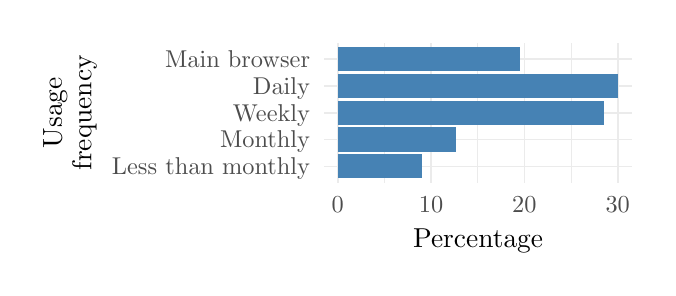
\begin{tikzpicture}[x=1pt,y=1pt]
\definecolor{fillColor}{RGB}{255,255,255}
\path[use as bounding box,fill=fillColor,fill opacity=0.00] (0,0) rectangle (224.04, 86.72);
\begin{scope}
\path[clip] (106.99, 30.77) rectangle (218.54, 81.22);
\definecolor{drawColor}{gray}{0.92}

\path[draw=drawColor,line width= 0.3pt,line join=round] (128.91, 30.77) --
	(128.91, 81.22);

\path[draw=drawColor,line width= 0.3pt,line join=round] (162.63, 30.77) --
	(162.63, 81.22);

\path[draw=drawColor,line width= 0.3pt,line join=round] (196.34, 30.77) --
	(196.34, 81.22);

\path[draw=drawColor,line width= 0.6pt,line join=round] (106.99, 36.59) --
	(218.54, 36.59);

\path[draw=drawColor,line width= 0.6pt,line join=round] (106.99, 46.30) --
	(218.54, 46.30);

\path[draw=drawColor,line width= 0.6pt,line join=round] (106.99, 56.00) --
	(218.54, 56.00);

\path[draw=drawColor,line width= 0.6pt,line join=round] (106.99, 65.70) --
	(218.54, 65.70);

\path[draw=drawColor,line width= 0.6pt,line join=round] (106.99, 75.40) --
	(218.54, 75.40);

\path[draw=drawColor,line width= 0.6pt,line join=round] (112.06, 30.77) --
	(112.06, 81.22);

\path[draw=drawColor,line width= 0.6pt,line join=round] (145.77, 30.77) --
	(145.77, 81.22);

\path[draw=drawColor,line width= 0.6pt,line join=round] (179.48, 30.77) --
	(179.48, 81.22);

\path[draw=drawColor,line width= 0.6pt,line join=round] (213.20, 30.77) --
	(213.20, 81.22);
\definecolor{fillColor}{RGB}{70,130,180}

\path[fill=fillColor] (112.06, 32.23) rectangle (142.40, 40.96);

\path[fill=fillColor] (112.06, 41.93) rectangle (154.67, 50.66);

\path[fill=fillColor] (112.06, 51.63) rectangle (208.27, 60.36);

\path[fill=fillColor] (112.06, 61.33) rectangle (213.47, 70.07);

\path[fill=fillColor] (112.06, 71.04) rectangle (177.93, 79.77);
\end{scope}
\begin{scope}
\path[clip] (  0.00,  0.00) rectangle (224.04, 86.72);
\definecolor{drawColor}{gray}{0.30}

\node[text=drawColor,anchor=base east,inner sep=0pt, outer sep=0pt, scale=  0.88] at (102.04, 33.56) {Less than monthly};

\node[text=drawColor,anchor=base east,inner sep=0pt, outer sep=0pt, scale=  0.88] at (102.04, 43.27) {Monthly};

\node[text=drawColor,anchor=base east,inner sep=0pt, outer sep=0pt, scale=  0.88] at (102.04, 52.97) {Weekly};

\node[text=drawColor,anchor=base east,inner sep=0pt, outer sep=0pt, scale=  0.88] at (102.04, 62.67) {Daily};

\node[text=drawColor,anchor=base east,inner sep=0pt, outer sep=0pt, scale=  0.88] at (102.04, 72.37) {Main browser};
\end{scope}
\begin{scope}
\path[clip] (  0.00,  0.00) rectangle (224.04, 86.72);
\definecolor{drawColor}{gray}{0.30}

\node[text=drawColor,anchor=base,inner sep=0pt, outer sep=0pt, scale=  0.88] at (112.06, 19.76) {0};

\node[text=drawColor,anchor=base,inner sep=0pt, outer sep=0pt, scale=  0.88] at (145.77, 19.76) {10};

\node[text=drawColor,anchor=base,inner sep=0pt, outer sep=0pt, scale=  0.88] at (179.48, 19.76) {20};

\node[text=drawColor,anchor=base,inner sep=0pt, outer sep=0pt, scale=  0.88] at (213.20, 19.76) {30};
\end{scope}
\begin{scope}
\path[clip] (  0.00,  0.00) rectangle (224.04, 86.72);
\definecolor{drawColor}{RGB}{0,0,0}

\node[text=drawColor,anchor=base,inner sep=0pt, outer sep=0pt, scale=  0.99] at (162.76,  7.44) {Percentage};
\end{scope}
\begin{scope}
\path[clip] (  0.00,  0.00) rectangle (224.04, 86.72);
\definecolor{drawColor}{RGB}{0,0,0}

\node[text=drawColor,rotate= 90.00,anchor=base,inner sep=0pt, outer sep=0pt, scale=  0.99] at ( 12.32, 56.00) {Usage};

\node[text=drawColor,rotate= 90.00,anchor=base,inner sep=0pt, outer sep=0pt, scale=  0.99] at ( 23.01, 56.00) {frequency};
\end{scope}
\end{tikzpicture}

    \caption{The usage frequency of Tor Browser among our respondents.  Almost
    half of our respondents use Tor Browser either daily or as their main
    browser.}
    \label{fig:tor-usage}
\end{figure}

\begin{figure}[t]
    \centering
    % Created by tikzDevice version 0.10.1 on 2018-01-12 15:55:52
% !TEX encoding = UTF-8 Unicode
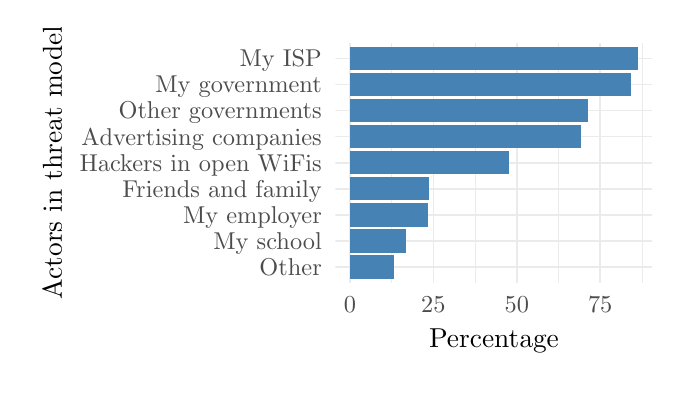
\begin{tikzpicture}[x=1pt,y=1pt]
\definecolor{fillColor}{RGB}{255,255,255}
\path[use as bounding box,fill=fillColor,fill opacity=0.00] (0,0) rectangle (231.26,122.86);
\begin{scope}
\path[clip] (111.23, 30.77) rectangle (225.76,117.36);
\definecolor{drawColor}{gray}{0.92}

\path[draw=drawColor,line width= 0.3pt,line join=round] (131.51, 30.77) --
	(131.51,117.36);

\path[draw=drawColor,line width= 0.3pt,line join=round] (161.66, 30.77) --
	(161.66,117.36);

\path[draw=drawColor,line width= 0.3pt,line join=round] (191.81, 30.77) --
	(191.81,117.36);

\path[draw=drawColor,line width= 0.3pt,line join=round] (221.96, 30.77) --
	(221.96,117.36);

\path[draw=drawColor,line width= 0.6pt,line join=round] (111.23, 36.42) --
	(225.76, 36.42);

\path[draw=drawColor,line width= 0.6pt,line join=round] (111.23, 45.83) --
	(225.76, 45.83);

\path[draw=drawColor,line width= 0.6pt,line join=round] (111.23, 55.24) --
	(225.76, 55.24);

\path[draw=drawColor,line width= 0.6pt,line join=round] (111.23, 64.65) --
	(225.76, 64.65);

\path[draw=drawColor,line width= 0.6pt,line join=round] (111.23, 74.07) --
	(225.76, 74.07);

\path[draw=drawColor,line width= 0.6pt,line join=round] (111.23, 83.48) --
	(225.76, 83.48);

\path[draw=drawColor,line width= 0.6pt,line join=round] (111.23, 92.89) --
	(225.76, 92.89);

\path[draw=drawColor,line width= 0.6pt,line join=round] (111.23,102.30) --
	(225.76,102.30);

\path[draw=drawColor,line width= 0.6pt,line join=round] (111.23,111.71) --
	(225.76,111.71);

\path[draw=drawColor,line width= 0.6pt,line join=round] (116.44, 30.77) --
	(116.44,117.36);

\path[draw=drawColor,line width= 0.6pt,line join=round] (146.59, 30.77) --
	(146.59,117.36);

\path[draw=drawColor,line width= 0.6pt,line join=round] (176.73, 30.77) --
	(176.73,117.36);

\path[draw=drawColor,line width= 0.6pt,line join=round] (206.88, 30.77) --
	(206.88,117.36);
\definecolor{fillColor}{RGB}{70,130,180}

\path[fill=fillColor] (116.44, 32.18) rectangle (132.22, 40.66);

\path[fill=fillColor] (116.44, 41.60) rectangle (136.81, 50.07);

\path[fill=fillColor] (116.44, 51.01) rectangle (144.81, 59.48);

\path[fill=fillColor] (116.44, 60.42) rectangle (145.04, 68.89);

\path[fill=fillColor] (116.44, 69.83) rectangle (173.88, 78.30);

\path[fill=fillColor] (116.44, 79.24) rectangle (199.96, 87.71);

\path[fill=fillColor] (116.44, 88.65) rectangle (202.48, 97.12);

\path[fill=fillColor] (116.44, 98.07) rectangle (218.04,106.54);

\path[fill=fillColor] (116.44,107.48) rectangle (220.56,115.95);
\end{scope}
\begin{scope}
\path[clip] (  0.00,  0.00) rectangle (231.26,122.86);
\definecolor{drawColor}{gray}{0.30}

\node[text=drawColor,anchor=base east,inner sep=0pt, outer sep=0pt, scale=  0.88] at (106.28, 33.39) {Other};

\node[text=drawColor,anchor=base east,inner sep=0pt, outer sep=0pt, scale=  0.88] at (106.28, 42.80) {My school};

\node[text=drawColor,anchor=base east,inner sep=0pt, outer sep=0pt, scale=  0.88] at (106.28, 52.21) {My employer};

\node[text=drawColor,anchor=base east,inner sep=0pt, outer sep=0pt, scale=  0.88] at (106.28, 61.62) {Friends and family};

\node[text=drawColor,anchor=base east,inner sep=0pt, outer sep=0pt, scale=  0.88] at (106.28, 71.04) {Hackers in open WiFis};

\node[text=drawColor,anchor=base east,inner sep=0pt, outer sep=0pt, scale=  0.88] at (106.28, 80.45) {Advertising companies};

\node[text=drawColor,anchor=base east,inner sep=0pt, outer sep=0pt, scale=  0.88] at (106.28, 89.86) {Other governments};

\node[text=drawColor,anchor=base east,inner sep=0pt, outer sep=0pt, scale=  0.88] at (106.28, 99.27) {My government};

\node[text=drawColor,anchor=base east,inner sep=0pt, outer sep=0pt, scale=  0.88] at (106.28,108.68) {My ISP};
\end{scope}
\begin{scope}
\path[clip] (  0.00,  0.00) rectangle (231.26,122.86);
\definecolor{drawColor}{gray}{0.30}

\node[text=drawColor,anchor=base,inner sep=0pt, outer sep=0pt, scale=  0.88] at (116.44, 19.76) {0};

\node[text=drawColor,anchor=base,inner sep=0pt, outer sep=0pt, scale=  0.88] at (146.59, 19.76) {25};

\node[text=drawColor,anchor=base,inner sep=0pt, outer sep=0pt, scale=  0.88] at (176.73, 19.76) {50};

\node[text=drawColor,anchor=base,inner sep=0pt, outer sep=0pt, scale=  0.88] at (206.88, 19.76) {75};
\end{scope}
\begin{scope}
\path[clip] (  0.00,  0.00) rectangle (231.26,122.86);
\definecolor{drawColor}{RGB}{0,0,0}

\node[text=drawColor,anchor=base,inner sep=0pt, outer sep=0pt, scale=  0.99] at (168.50,  7.44) {Percentage};
\end{scope}
\begin{scope}
\path[clip] (  0.00,  0.00) rectangle (231.26,122.86);
\definecolor{drawColor}{RGB}{0,0,0}

\node[text=drawColor,rotate= 90.00,anchor=base,inner sep=0pt, outer sep=0pt, scale=  0.99] at ( 12.32, 74.07) {Actors in threat model};
\end{scope}
\end{tikzpicture}

    \caption{The threat actors that our respondents seek to protect themselves
        from by using Tor Browser.}
    \label{fig:tor-threats}
\end{figure}

People who selected ``Other'' gave a variety of responses.  A number of
respondents specifically pointed out Google and Facebook.  ISPs, backbone ISPs,
and web sites were another common theme.  A number of respondents are struggling
with personal threats that include identity theft, targeted harassment, and
stalking.  Research is another common theme: Several respondents want to learn
about a topic without revealing their interest in it.  Some respondents use Tor
for search engine optimization, computer security research, and to research
medical conditions.  Finally, Tor provides technical advantages that don't
involve a threat actor.  Some respondents want IPv6 connectivity, evasion of
geographical content restrictions, and access to onion services.  A small number
of respondents are only interested in technical aspects other than privacy.  One
respondent stated that they don't need anonymity themselves but instead use Tor
to provide cover traffic for ``people who need protection.''

\subsubsection{Quantifying anonymity is hard}

The degree of anonymity that protects a Tor user in a given situation depends on
a number of variables including her guard relay, intermediate autonomous systems
between the user and her destination, and other people that are using Tor at the
same time, just to name a few.  Unlike other anonymity tools such as
JAP~\cite{jap}, Tor Browser makes no attempt to display the degree of anonymity
it believes it can provide.  Asked about how well Tor works for them, one
of our participants explained:

\begin{displayquote}[P12]
In terms of the anonymity, you can't really tell\dots That's fairly opaque, so I
can't even tell how effective that's working, or whether it is\dots
\end{displayquote}

Quantifying anonymity in a real-world setting is complex, error-prone, and often
misleading.  What's more, Tor Browser does not have available all the data it
needs to quantify its user's anonymity---an ``anonymity meter'' may therefore
create more problems than it solves.

\subsubsection{Users like a view under the hood}

\begin{figure}[t]
    \centering
    \includegraphics[width=\linewidth]{figures/tor-button-screenshot.jpg}
    \caption{A click on the onion icon reveals the Tor relays that constitute
    the circuit that was used to fetch the current page.}
    \label{fig:tor-button}
\end{figure}

Several of our participants enjoyed Tor Browser's visual feedback, illustrated
in Figure~\ref{fig:tor-button}, that shows the circuit that is used for a given
site.  One interviewee expressed delight about the interface:

\begin{displayquote}[P08]
I love how I can monitor the network through this little kind of bar that comes
up.
\end{displayquote}

Not satisfied with seeing only the current circuit, some participants wished it
were easier to learn what else is happening behind the scenes:

\begin{displayquote}[P02]
{[It]} would be nice to have some kind of application, something on that browser,
that gives you an impression of\dots what the Tor Browser's actually doing.
\end{displayquote}

Finding the right balance between what information to show and what to hide is
challenging in itself, and only exacerbated by Tor's heterogeneous user base:
While technical users may appreciate a look ``under the hood,'' non-technical
users, who often use Tor as a tool to get a specific job
done~\cite[\S~4.3.2]{Gallagher2017a}, can easily feel bewildered and
overwhelmed.  One aspect in which more transparency could indeed benefit Tor's
entire user base is when websites don't load, as suggested by one participant:

\begin{displayquote}[P05]
\dots maybe some sort of graphical representation of is the circuit still
being built, or is the circuit built, and the site isn't responding at all to
the third relay?
\end{displayquote}

\subsubsection{Users lament speed, user interface, and CAPTCHAs}

Perhaps the most prevalent issue is, still, browsing speed:

\begin{displayquote}[P01]
The speed of it is problematic; sometimes I have a path that allows me to watch
streaming full HD YouTube videos, and the next time, five minutes later, I'm
barely getting kilobytes through.
\end{displayquote}

Occasionally Tor is preceded by its reputation, preparing users for what to
expect:

\begin{displayquote}[P03]
I didn't think it was as slow as people say it was. People said it would be much
slower experience but\ldots a little bit slower, but it didn't matter for the
things that I was doing.
\end{displayquote}

In addition to the perceived slowness, several participants lamented the
old-fashioned user interface.  Tor Browser's looks were described as ``it felt
like it was about five years outdated,'' ``it looked like I was in 1982,'' and
``I think the colors look a bit old fashioned and in the former Soviet Union.''
Interestingly, one participant drew the opposite conclusion, expressing that the
antiquated user interface evoked trust:

\begin{displayquote}[P02]
At the same time I thought\ldots it gave them a certain amount of credibility,
like they weren't building this for the looks, but they were building it for
functionality\ldots  At the same time, as I thought it was outdated in terms of
how it looked, I also thought it was sort of genuine in a way.
\end{displayquote}

Orthogonal Tor's speed and user interface, the browsing experience occasionally
suffers.  Relying on naive, IP address-based metrics of ``maliciousness,'' some
content delivery networks such as Cloudflare label Tor exit relays as malicious
which results in Tor users having to solve (sometimes multiple) CAPTCHAs before
being granted access to a website.  In 2016, Khattak \ea documented the issue
for a number of content providers~\cite{Khattak2016a}.  One interviewee summed
up the situation as follows:

\begin{displayquote}[P06]
It is still sometimes challenging using some everyday services, because of
CAPTCHAs and those things, but I also understand that's not so much to do with
Tor, but to do with the creators of those web sites.
\end{displayquote}

\subsubsection{Tor Browser provides security, privacy, and control}

Let's turn to the advantages that our interviewees see in Tor Browser.  It comes
as no surprise that the main benefit of Tor Browser is the increase in privacy
and security, brought up by practically all of our participants.  One of our
more technical interviewees further distinguished between security and privacy.
Asked about if they feel safer when using Tor, they responded:

\begin{displayquote}[P06]
In a privacy sense, I do. In a security sense\ldots I don't assume that Tor is
protecting me from all of the vulnerabilities or exploits that I might
encounter\ldots
\end{displayquote}

Besides the obvious improvement in security and privacy, a defining aspect of
Tor is that it puts its users back in control, or, as one of our participants
eloquently put it:

\begin{displayquote}[P02]
I feel like I'm more in control of my internet experience that way, I'm not sort
of like a will-less victim of what other people want to do with me, so I feel
I'm more empowered and have more agency when I use the Tor Browser.
\end{displayquote}

\subsection{Onion service usage}

We now move on to results specific to onion services.

\subsubsection{Usage frequency}

The usage frequency of onion services is almost uniformly distributed among our
respondents; 24\% use onion sites less than once a month, 22\% use them about
monthly, 25\% weekly, and 23\% daily.  The remaining 6\% has never used an onion
service before.

The majority of our respondents (61.8\%) has used onion services for purposes
other than web browsing before.  Several protocols such as the chat application
Ricochet~\cite{ricochet} and the file sharing application
OnionShare~\cite{onionshare} were purpose-built on top of onion services while
existing TCP-based tools such as SSH can also be used with onion addresses
instead of traditional IP addresses.  Almost one third (29.7\%) of our
participants use onion service for non-browsing activities at least once a week.

But why do Tor users browse onion services in the first place?
Figure~\ref{fig:onion-usage} provides an answer.  The majority uses onion
services because of the additional anonymity (70\%) and the additional security
(61\%).  For 46\% it is the only way to access some content they enjoy, so using
onion services is a necessity.  27\% of our respondents found themselves curious
about the ``Dark Web'' and set out to find their own answer and 19\%
occasionally stumble upon links to onion services in their day-to-day browsing
activity.  Respondents who selected ``Other'' gave a variety of reasons, the
most predominant of which was the ability to set up a TCP service behind a NAT
device.  That way, it is possible to run an SSH server in a home network that
has neither a permanent IP address, nor port forwarding.  Other noteworthy
respondents use onion services to reduce the load on exit relays, to do
technical research, and to access sites that are otherwise unavailable.

\begin{figure}[t]
    \centering
    % Created by tikzDevice version 0.10.1 on 2018-01-12 16:14:57
% !TEX encoding = UTF-8 Unicode
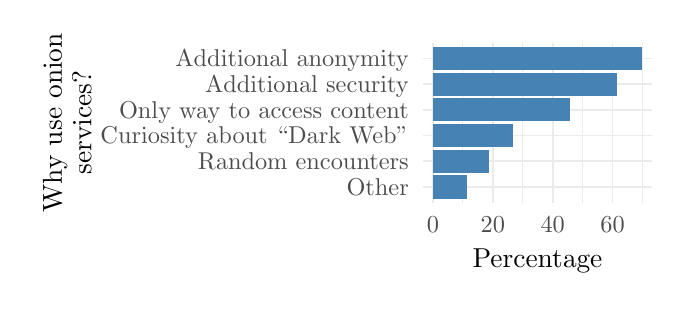
\begin{tikzpicture}[x=1pt,y=1pt]
\definecolor{fillColor}{RGB}{255,255,255}
\path[use as bounding box,fill=fillColor,fill opacity=0.00] (0,0) rectangle (231.26, 93.95);
\begin{scope}
\path[clip] (142.68, 30.77) rectangle (225.76, 88.45);
\definecolor{drawColor}{gray}{0.92}

\path[draw=drawColor,line width= 0.3pt,line join=round] (157.27, 30.77) --
	(157.27, 88.45);

\path[draw=drawColor,line width= 0.3pt,line join=round] (178.90, 30.77) --
	(178.90, 88.45);

\path[draw=drawColor,line width= 0.3pt,line join=round] (200.54, 30.77) --
	(200.54, 88.45);

\path[draw=drawColor,line width= 0.3pt,line join=round] (222.17, 30.77) --
	(222.17, 88.45);

\path[draw=drawColor,line width= 0.6pt,line join=round] (142.68, 36.35) --
	(225.76, 36.35);

\path[draw=drawColor,line width= 0.6pt,line join=round] (142.68, 45.66) --
	(225.76, 45.66);

\path[draw=drawColor,line width= 0.6pt,line join=round] (142.68, 54.96) --
	(225.76, 54.96);

\path[draw=drawColor,line width= 0.6pt,line join=round] (142.68, 64.26) --
	(225.76, 64.26);

\path[draw=drawColor,line width= 0.6pt,line join=round] (142.68, 73.57) --
	(225.76, 73.57);

\path[draw=drawColor,line width= 0.6pt,line join=round] (142.68, 82.87) --
	(225.76, 82.87);

\path[draw=drawColor,line width= 0.6pt,line join=round] (146.45, 30.77) --
	(146.45, 88.45);

\path[draw=drawColor,line width= 0.6pt,line join=round] (168.09, 30.77) --
	(168.09, 88.45);

\path[draw=drawColor,line width= 0.6pt,line join=round] (189.72, 30.77) --
	(189.72, 88.45);

\path[draw=drawColor,line width= 0.6pt,line join=round] (211.35, 30.77) --
	(211.35, 88.45);
\definecolor{fillColor}{RGB}{70,130,180}

\path[fill=fillColor] (146.45, 32.17) rectangle (158.77, 40.54);

\path[fill=fillColor] (146.45, 41.47) rectangle (166.57, 49.84);

\path[fill=fillColor] (146.45, 50.77) rectangle (175.40, 59.15);

\path[fill=fillColor] (146.45, 60.08) rectangle (196.12, 68.45);

\path[fill=fillColor] (146.45, 69.38) rectangle (212.96, 77.75);

\path[fill=fillColor] (146.45, 78.68) rectangle (221.99, 87.06);
\end{scope}
\begin{scope}
\path[clip] (  0.00,  0.00) rectangle (231.26, 93.95);
\definecolor{drawColor}{gray}{0.30}

\node[text=drawColor,anchor=base east,inner sep=0pt, outer sep=0pt, scale=  0.88] at (137.73, 33.32) {Other};

\node[text=drawColor,anchor=base east,inner sep=0pt, outer sep=0pt, scale=  0.88] at (137.73, 42.63) {Random encounters};

\node[text=drawColor,anchor=base east,inner sep=0pt, outer sep=0pt, scale=  0.88] at (137.73, 51.93) {Curiosity about ``Dark Web''};

\node[text=drawColor,anchor=base east,inner sep=0pt, outer sep=0pt, scale=  0.88] at (137.73, 61.23) {Only way to access content};

\node[text=drawColor,anchor=base east,inner sep=0pt, outer sep=0pt, scale=  0.88] at (137.73, 70.54) {Additional security};

\node[text=drawColor,anchor=base east,inner sep=0pt, outer sep=0pt, scale=  0.88] at (137.73, 79.84) {Additional anonymity};
\end{scope}
\begin{scope}
\path[clip] (  0.00,  0.00) rectangle (231.26, 93.95);
\definecolor{drawColor}{gray}{0.30}

\node[text=drawColor,anchor=base,inner sep=0pt, outer sep=0pt, scale=  0.88] at (146.45, 19.76) {0};

\node[text=drawColor,anchor=base,inner sep=0pt, outer sep=0pt, scale=  0.88] at (168.09, 19.76) {20};

\node[text=drawColor,anchor=base,inner sep=0pt, outer sep=0pt, scale=  0.88] at (189.72, 19.76) {40};

\node[text=drawColor,anchor=base,inner sep=0pt, outer sep=0pt, scale=  0.88] at (211.35, 19.76) {60};
\end{scope}
\begin{scope}
\path[clip] (  0.00,  0.00) rectangle (231.26, 93.95);
\definecolor{drawColor}{RGB}{0,0,0}

\node[text=drawColor,anchor=base,inner sep=0pt, outer sep=0pt, scale=  0.99] at (184.22,  7.44) {Percentage};
\end{scope}
\begin{scope}
\path[clip] (  0.00,  0.00) rectangle (231.26, 93.95);
\definecolor{drawColor}{RGB}{0,0,0}

\node[text=drawColor,rotate= 90.00,anchor=base,inner sep=0pt, outer sep=0pt, scale=  0.99] at ( 12.32, 59.61) {Why use onion};

\node[text=drawColor,rotate= 90.00,anchor=base,inner sep=0pt, outer sep=0pt, scale=  0.99] at ( 23.01, 59.61) {services?};
\end{scope}
\end{tikzpicture}

    \caption{Our respondents' (multiple choice) reasons for using onion
    services.}
    \label{fig:onion-usage}
\end{figure}

\subsubsection{Mental models}

We asked our participants to draw sketches of how they believe Tor and onion
services work.\footnote{All sketches are available online at
\url{https://nymity.ch/onion-services/mental-models/}.}   Everybody drew a
sketch of Tor but some didn't draw onion services because they had no mental
model of it.  Interestingly, all participants understood that bouncing network
traffic across several relays is key to Tor's anonymity, as evidenced by
Figure~\ref{fig:tor-sketch} that stems from a participant with no technical
background.\footnote{Nevertheless the sketch got two details wrong: the number
of hops in a Tor circuit is three and the circuit's forward and reverse path are
identical.}  Analogously, most of our participants understood that network
traffic does not leave the Tor network when connecting to onion services.
Figure~\ref{fig:os-sketch} illustrates an example, again drawn by a
non-technical participant.  The last hop in the circuit is an onion, correctly
suggesting that network traffic does not leave the Tor network.

\begin{figure}[t]
    \centering

    \begin{subfigure}[t]{\linewidth}
        \centering
        \includegraphics[width=0.8\linewidth]{figures/tor-sketch.jpg}
        \subcaption{A non-technical interview subject's sketch of how they
        believe Tor works.  The participant correctly understands the concept of
        bouncing network traffic over several hops.}
        \label{fig:tor-sketch}
    \end{subfigure}

    \begin{subfigure}[t]{\linewidth}
        \centering
        \includegraphics[width=0.8\linewidth]{figures/os-sketch.jpg}
        \subcaption{A non-technical interview subject's sketch of their mental
        model of an onion service.  Instead of a web site, the final hop is
        another Tor hop.}
        \label{fig:os-sketch}
    \end{subfigure}

    \caption{Sketches of two different, non-technical interview participants of
    how Tor works (top) and how onion services work (bottom).}
\end{figure}

Some of our interviewees did not distinguish disguising their IP address from
disguising their real-world identity, and instead used the umbrella term of
``anonymity'' to refer to both concepts.  This conflation of concepts paints an
incomplete picture of the security and privacy guarantees that Tor provides,
as evidenced by one participant's question:

\begin{displayquote}[P07]
What's the point of going to Facebook using onion services when their business
model is still about collecting your data?
\end{displayquote}

There is merit in using Facebook's onion service.  While the company obviously
knows who is logging in, they do not know Tor users' location, operating system,
or browser details.  On top of that, users get end-to-end security as well as
self-authenticating names.  These benefits are difficult to convey to
non-technical users and even experts sometimes advocate an ``all or nothing''
approach to online anonymity.

\subsubsection{Onion service discovery is a mess}

Recall that onion services are private by default, leaving it up to their
operator to disseminate the domain.  Established search engines such as Google
are therefore inadequate to find content on onion services.  We wanted to find
out how our respondents discover onion services.
Figure~\ref{fig:onion-discovery} illustrates the results.  The three most
popular ways of discovering new onion sites, all approximating 50\%, are social
networking sites such as Twitter and Reddit, the list of search engines such as
Ahmia\footnote{Ahmia.fi is an onion site search engine that crawls
user-submitted onion domains.  It publishes the list of all indexed onion
services at \url{https://ahmia.fi/onions/}.}, and randomly encountering links
when browsing the web.

While significantly less popular, discovering onion domains through friends and
family has the advantage of trust.  Some of our interview participant indicated
that they heavily rely on this distribution method simply because they can trust
the origin.  Finally, a mere 4\% indicated that they are not interested in
learning about new onion services.

Respondents who selected ``Other'' predominantly brought up
independently-maintained lists of onion services and aggregators.  A noteworthy
example is the Hidden Wiki.

\begin{figure}[t]
    \centering
    % Created by tikzDevice version 0.10.1 on 2018-01-12 16:15:03
% !TEX encoding = UTF-8 Unicode
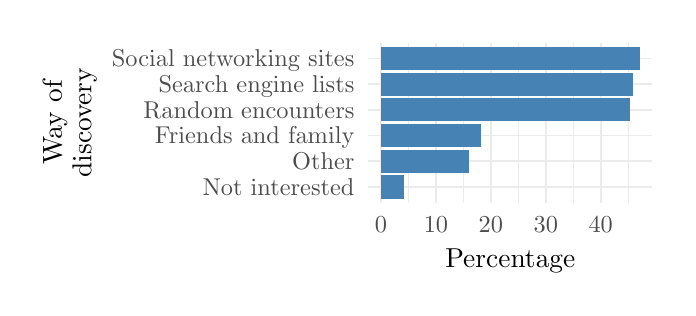
\begin{tikzpicture}[x=1pt,y=1pt]
\definecolor{fillColor}{RGB}{255,255,255}
\path[use as bounding box,fill=fillColor,fill opacity=0.00] (0,0) rectangle (231.26, 93.95);
\begin{scope}
\path[clip] (123.02, 30.77) rectangle (225.76, 88.45);
\definecolor{drawColor}{gray}{0.92}

\path[draw=drawColor,line width= 0.3pt,line join=round] (137.61, 30.77) --
	(137.61, 88.45);

\path[draw=drawColor,line width= 0.3pt,line join=round] (157.46, 30.77) --
	(157.46, 88.45);

\path[draw=drawColor,line width= 0.3pt,line join=round] (177.31, 30.77) --
	(177.31, 88.45);

\path[draw=drawColor,line width= 0.3pt,line join=round] (197.16, 30.77) --
	(197.16, 88.45);

\path[draw=drawColor,line width= 0.3pt,line join=round] (217.00, 30.77) --
	(217.00, 88.45);

\path[draw=drawColor,line width= 0.6pt,line join=round] (123.02, 36.35) --
	(225.76, 36.35);

\path[draw=drawColor,line width= 0.6pt,line join=round] (123.02, 45.66) --
	(225.76, 45.66);

\path[draw=drawColor,line width= 0.6pt,line join=round] (123.02, 54.96) --
	(225.76, 54.96);

\path[draw=drawColor,line width= 0.6pt,line join=round] (123.02, 64.26) --
	(225.76, 64.26);

\path[draw=drawColor,line width= 0.6pt,line join=round] (123.02, 73.57) --
	(225.76, 73.57);

\path[draw=drawColor,line width= 0.6pt,line join=round] (123.02, 82.87) --
	(225.76, 82.87);

\path[draw=drawColor,line width= 0.6pt,line join=round] (127.69, 30.77) --
	(127.69, 88.45);

\path[draw=drawColor,line width= 0.6pt,line join=round] (147.54, 30.77) --
	(147.54, 88.45);

\path[draw=drawColor,line width= 0.6pt,line join=round] (167.38, 30.77) --
	(167.38, 88.45);

\path[draw=drawColor,line width= 0.6pt,line join=round] (187.23, 30.77) --
	(187.23, 88.45);

\path[draw=drawColor,line width= 0.6pt,line join=round] (207.08, 30.77) --
	(207.08, 88.45);
\definecolor{fillColor}{RGB}{70,130,180}

\path[fill=fillColor] (127.69, 32.17) rectangle (135.96, 40.54);

\path[fill=fillColor] (127.69, 41.47) rectangle (159.33, 49.84);

\path[fill=fillColor] (127.69, 50.77) rectangle (163.85, 59.15);

\path[fill=fillColor] (127.69, 60.08) rectangle (217.70, 68.45);

\path[fill=fillColor] (127.69, 69.38) rectangle (218.83, 77.75);

\path[fill=fillColor] (127.69, 78.68) rectangle (221.09, 87.06);
\end{scope}
\begin{scope}
\path[clip] (  0.00,  0.00) rectangle (231.26, 93.95);
\definecolor{drawColor}{gray}{0.30}

\node[text=drawColor,anchor=base east,inner sep=0pt, outer sep=0pt, scale=  0.88] at (118.07, 33.32) {Not interested};

\node[text=drawColor,anchor=base east,inner sep=0pt, outer sep=0pt, scale=  0.88] at (118.07, 42.63) {Other};

\node[text=drawColor,anchor=base east,inner sep=0pt, outer sep=0pt, scale=  0.88] at (118.07, 51.93) {Friends and family};

\node[text=drawColor,anchor=base east,inner sep=0pt, outer sep=0pt, scale=  0.88] at (118.07, 61.23) {Random encounters};

\node[text=drawColor,anchor=base east,inner sep=0pt, outer sep=0pt, scale=  0.88] at (118.07, 70.54) {Search engine lists};

\node[text=drawColor,anchor=base east,inner sep=0pt, outer sep=0pt, scale=  0.88] at (118.07, 79.84) {Social networking sites};
\end{scope}
\begin{scope}
\path[clip] (  0.00,  0.00) rectangle (231.26, 93.95);
\definecolor{drawColor}{gray}{0.30}

\node[text=drawColor,anchor=base,inner sep=0pt, outer sep=0pt, scale=  0.88] at (127.69, 19.76) {0};

\node[text=drawColor,anchor=base,inner sep=0pt, outer sep=0pt, scale=  0.88] at (147.54, 19.76) {10};

\node[text=drawColor,anchor=base,inner sep=0pt, outer sep=0pt, scale=  0.88] at (167.38, 19.76) {20};

\node[text=drawColor,anchor=base,inner sep=0pt, outer sep=0pt, scale=  0.88] at (187.23, 19.76) {30};

\node[text=drawColor,anchor=base,inner sep=0pt, outer sep=0pt, scale=  0.88] at (207.08, 19.76) {40};
\end{scope}
\begin{scope}
\path[clip] (  0.00,  0.00) rectangle (231.26, 93.95);
\definecolor{drawColor}{RGB}{0,0,0}

\node[text=drawColor,anchor=base,inner sep=0pt, outer sep=0pt, scale=  0.99] at (174.39,  7.44) {Percentage};
\end{scope}
\begin{scope}
\path[clip] (  0.00,  0.00) rectangle (231.26, 93.95);
\definecolor{drawColor}{RGB}{0,0,0}

\node[text=drawColor,rotate= 90.00,anchor=base,inner sep=0pt, outer sep=0pt, scale=  0.99] at ( 12.32, 59.61) {Way of};

\node[text=drawColor,rotate= 90.00,anchor=base,inner sep=0pt, outer sep=0pt, scale=  0.99] at ( 23.01, 59.61) {discovery};
\end{scope}
\end{tikzpicture}

    \caption{Our respondents' (multiple choice) methods of discovering onion
    services.}
    \label{fig:onion-discovery}
\end{figure}

The next question in our survey then asked if our respondents are satisfied with
the way they discover onion services.  60\% selected ``Yes'' while 40\% selected
``No.'' Some respondents who selected ``Yes'' brought up that they have no
interest in learning about new onion services, in part because they only use a
small set of onion services.  Among the people who are not satisfied, the most
prominent complaint was about broken links on onion site lists.  There is
non-trivial churn among onion sites and our respondents were frustrated that
existing lists are typically not curated and contain many dead links.

Many respondents were not aware of search engines such as ahmia.fi.  Among those
that were, many were not satisfied with both the search results and the number
of indexed onion sites.  Unsurprisingly, a ``Google for onion sites'' was a
frequent wish.

Several respondents were unhappy with existing aggregators.  In addition to
broken links, some distrust lists because they occasionally contain scam and
phishing sites.  The difficulty of telling apart two given onion domain names
exacerbates this issue.  Another common wish for aggregators was for them to be
more verbose in their description of onion sites.  In particular, some
respondents want to avoid illegal and pornographic content, which is often
difficult if the description is vague and the onion domain reveals nothing about
its content.

Many respondents expressed frustration about the difficulty of finding out if
site X also provides a corresponding onion service.  A common wish was to have
site X list its onion service prominently in a footer.  Ironically, some
respondents were surprised that torproject.org has a corresponding onion site --
they couldn't find it on the web site.

Interestingly, some respondents voiced frustration about various usability
issues, but mentioned in the same sentence that this is an inherent trade-off of
privacy technology, suggesting that there is nothing that can be done about it.

\subsubsection{Tools help managing the onion service domain format}

% An unrelated yet hardly unexpected source of confusion is the domain format of
% onion services.  Some users have come to believe that the seemingly-random
% characters in onion domains is the reason why onion services are anonymous.
% Accordingly, these users also believe that vanity domains are ``less anonymous''
% because part of their domains is clearly not random.

Conventional domains are designed to be easy to remember and recognize.  But how
do users handle the randomly-generated onion domains?  Question 3.8 in our
survey asked exactly that, with the responses being illustrated in
Figure~\ref{fig:onion-domain-mgmt}.

\begin{figure}[t]
    \centering
    % Created by tikzDevice version 0.10.1 on 2018-02-09 14:36:33
% !TEX encoding = UTF-8 Unicode
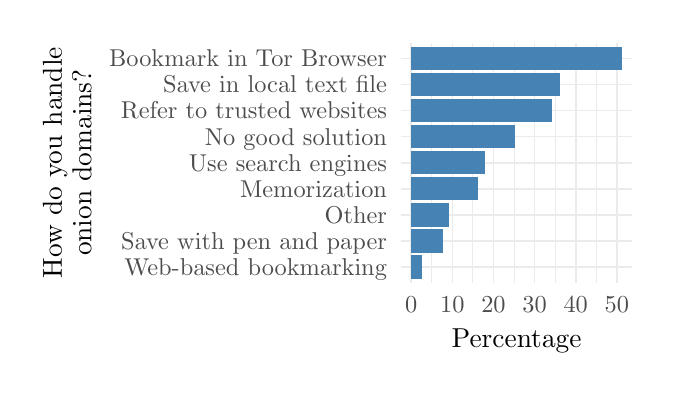
\begin{tikzpicture}[x=1pt,y=1pt]
\definecolor{fillColor}{RGB}{255,255,255}
\path[use as bounding box,fill=fillColor,fill opacity=0.00] (0,0) rectangle (224.04,122.86);
\begin{scope}
\path[clip] (134.78, 30.77) rectangle (218.54,117.36);
\definecolor{drawColor}{gray}{0.92}

\path[draw=drawColor,line width= 0.3pt,line join=round] (146.02, 30.77) --
	(146.02,117.36);

\path[draw=drawColor,line width= 0.3pt,line join=round] (160.88, 30.77) --
	(160.88,117.36);

\path[draw=drawColor,line width= 0.3pt,line join=round] (175.74, 30.77) --
	(175.74,117.36);

\path[draw=drawColor,line width= 0.3pt,line join=round] (190.61, 30.77) --
	(190.61,117.36);

\path[draw=drawColor,line width= 0.3pt,line join=round] (205.47, 30.77) --
	(205.47,117.36);

\path[draw=drawColor,line width= 0.6pt,line join=round] (134.78, 36.42) --
	(218.54, 36.42);

\path[draw=drawColor,line width= 0.6pt,line join=round] (134.78, 45.83) --
	(218.54, 45.83);

\path[draw=drawColor,line width= 0.6pt,line join=round] (134.78, 55.24) --
	(218.54, 55.24);

\path[draw=drawColor,line width= 0.6pt,line join=round] (134.78, 64.65) --
	(218.54, 64.65);

\path[draw=drawColor,line width= 0.6pt,line join=round] (134.78, 74.07) --
	(218.54, 74.07);

\path[draw=drawColor,line width= 0.6pt,line join=round] (134.78, 83.48) --
	(218.54, 83.48);

\path[draw=drawColor,line width= 0.6pt,line join=round] (134.78, 92.89) --
	(218.54, 92.89);

\path[draw=drawColor,line width= 0.6pt,line join=round] (134.78,102.30) --
	(218.54,102.30);

\path[draw=drawColor,line width= 0.6pt,line join=round] (134.78,111.71) --
	(218.54,111.71);

\path[draw=drawColor,line width= 0.6pt,line join=round] (138.58, 30.77) --
	(138.58,117.36);

\path[draw=drawColor,line width= 0.6pt,line join=round] (153.45, 30.77) --
	(153.45,117.36);

\path[draw=drawColor,line width= 0.6pt,line join=round] (168.31, 30.77) --
	(168.31,117.36);

\path[draw=drawColor,line width= 0.6pt,line join=round] (183.17, 30.77) --
	(183.17,117.36);

\path[draw=drawColor,line width= 0.6pt,line join=round] (198.04, 30.77) --
	(198.04,117.36);

\path[draw=drawColor,line width= 0.6pt,line join=round] (212.90, 30.77) --
	(212.90,117.36);
\definecolor{fillColor}{RGB}{70,130,180}

\path[fill=fillColor] (138.58, 32.18) rectangle (142.54, 40.66);

\path[fill=fillColor] (138.58, 41.60) rectangle (150.15, 50.07);

\path[fill=fillColor] (138.58, 51.01) rectangle (152.13, 59.48);

\path[fill=fillColor] (138.58, 60.42) rectangle (162.84, 68.89);

\path[fill=fillColor] (138.58, 69.83) rectangle (165.10, 78.30);

\path[fill=fillColor] (138.58, 79.24) rectangle (176.10, 87.71);

\path[fill=fillColor] (138.58, 88.65) rectangle (189.36, 97.12);

\path[fill=fillColor] (138.58, 98.07) rectangle (192.45,106.54);

\path[fill=fillColor] (138.58,107.48) rectangle (214.73,115.95);
\end{scope}
\begin{scope}
\path[clip] (  0.00,  0.00) rectangle (224.04,122.86);
\definecolor{drawColor}{gray}{0.30}

\node[text=drawColor,anchor=base east,inner sep=0pt, outer sep=0pt, scale=  0.88] at (129.83, 33.39) {Web-based bookmarking};

\node[text=drawColor,anchor=base east,inner sep=0pt, outer sep=0pt, scale=  0.88] at (129.83, 42.80) {Save with pen and paper};

\node[text=drawColor,anchor=base east,inner sep=0pt, outer sep=0pt, scale=  0.88] at (129.83, 52.21) {Other};

\node[text=drawColor,anchor=base east,inner sep=0pt, outer sep=0pt, scale=  0.88] at (129.83, 61.62) {Memorization};

\node[text=drawColor,anchor=base east,inner sep=0pt, outer sep=0pt, scale=  0.88] at (129.83, 71.04) {Use search engines};

\node[text=drawColor,anchor=base east,inner sep=0pt, outer sep=0pt, scale=  0.88] at (129.83, 80.45) {No good solution};

\node[text=drawColor,anchor=base east,inner sep=0pt, outer sep=0pt, scale=  0.88] at (129.83, 89.86) {Refer to trusted websites};

\node[text=drawColor,anchor=base east,inner sep=0pt, outer sep=0pt, scale=  0.88] at (129.83, 99.27) {Save in local text file};

\node[text=drawColor,anchor=base east,inner sep=0pt, outer sep=0pt, scale=  0.88] at (129.83,108.68) {Bookmark in Tor Browser};
\end{scope}
\begin{scope}
\path[clip] (  0.00,  0.00) rectangle (224.04,122.86);
\definecolor{drawColor}{gray}{0.30}

\node[text=drawColor,anchor=base,inner sep=0pt, outer sep=0pt, scale=  0.88] at (138.58, 19.76) {0};

\node[text=drawColor,anchor=base,inner sep=0pt, outer sep=0pt, scale=  0.88] at (153.45, 19.76) {10};

\node[text=drawColor,anchor=base,inner sep=0pt, outer sep=0pt, scale=  0.88] at (168.31, 19.76) {20};

\node[text=drawColor,anchor=base,inner sep=0pt, outer sep=0pt, scale=  0.88] at (183.17, 19.76) {30};

\node[text=drawColor,anchor=base,inner sep=0pt, outer sep=0pt, scale=  0.88] at (198.04, 19.76) {40};

\node[text=drawColor,anchor=base,inner sep=0pt, outer sep=0pt, scale=  0.88] at (212.90, 19.76) {50};
\end{scope}
\begin{scope}
\path[clip] (  0.00,  0.00) rectangle (224.04,122.86);
\definecolor{drawColor}{RGB}{0,0,0}

\node[text=drawColor,anchor=base,inner sep=0pt, outer sep=0pt, scale=  0.99] at (176.66,  7.44) {Percentage};
\end{scope}
\begin{scope}
\path[clip] (  0.00,  0.00) rectangle (224.04,122.86);
\definecolor{drawColor}{RGB}{0,0,0}

\node[text=drawColor,rotate= 90.00,anchor=base,inner sep=0pt, outer sep=0pt, scale=  0.99] at ( 12.32, 74.07) {How do you handle};

\node[text=drawColor,rotate= 90.00,anchor=base,inner sep=0pt, outer sep=0pt, scale=  0.99] at ( 23.01, 74.07) {onion domains?};
\end{scope}
\end{tikzpicture}

    \caption{The strategies that our respondents use to handle onion domains.
    More than half use bookmarks inside of Tor Browser and a quarter thinks that
    there's no good solution.}
    \label{fig:onion-domain-mgmt}
\end{figure}

Most respondents use bookmarks inside Tor Browser for onion domains.  While
convenient, it leaves a trace of (presumably) visited sites on one's computer.
One of Tor Browser's security requirements is ``disk avoidance,'' \ie, the
browser must not write anything to disk that would reveal the user's browsing
history~\cite[\S~2.1]{Perry2017a}.  Bookmarking links is a violation of this
security requirement.  Many of our respondents were aware of this issue.  About
a dozen respondents who selected ``Other'' stated that they store onion domains
encryptedly---either in a text file or in their password manager.

Somewhat less popular is saving onion domains in local text files (36\%),
getting them from trusted web sites (34\%), use search engines (18\%), memorize
domains (16\%), use some other techniques (9\%) or employ pen and paper (8\%).
Notably, one quarter of our respondents does not have a good solution to the
problem.  Given the alarming number of (possibly insecure) home-baked solutions,
a Tor Browser extension may be warranted to approach the problem.

The next question in our survey asked if our respondents expect the
next-generation domain format to change their browsing habits.  Interestingly,
only 17\% expect to have their browsing habits changed while 83\% don't.  Among
the respondents who selected ``Yes,'' many expressed that they memorize a small
number of onion domains (such as Facebook's), which will no longer be possible.
People who selected ``No'' mostly bring up that they treat onion domains as
opaque identifiers that they handle via tools such as bookmarks.  These results
suggest that the current state is dire, yet not expected to get much worse with
the new domain format.

Problematic:
``I only memorize the first part of the domain''

``If there isn't some cognizable word at the start, it'll be more difficult for
me to determine if I'm going to the correct domain or a scam. I may end up going
to less .onion sites as a result.''

\subsubsection{Onion service operation}

A survey question block on onion service operation shed light on the reasons for
running onion services and what sort of issues users face when doing so.  40\%
of our respondents once set up an onion service.  Among the respondents who
never have, 31\% have considered doing so while 30\% have never even considered
it.  Interestingly, 79\% of operators have run an onion service for private use
while 53\% have run them for the public.

Figure~\ref{fig:onion-operation-reasons} gives an overview of the reasons for
running onion services.  Interestingly, the extra security properties overshadow
the anonymity properties of onion services.  Another particularly popular reason
is NAT traversal---many respondents noted that onion services allow them to
expose a TCP service in their home network despite being behind a NAT device.
Finally, some people run onion service indirectly because third-party tools such
as OnionShare~\cite{onionshare} or Ricochet~\cite{ricochet} are built on top of
them.  Onion services can have clear benefits for businesses as well as
evidenced by one respondent who wrote on onion services: ``We use it for
delivering updates to our router to customers securely and without leaking
metadata.''

\begin{figure}[t]
    \centering
    % Created by tikzDevice version 0.10.1 on 2018-02-09 14:48:38
% !TEX encoding = UTF-8 Unicode
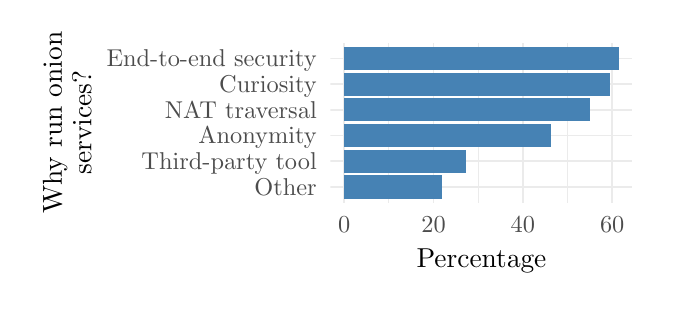
\begin{tikzpicture}[x=1pt,y=1pt]
\definecolor{fillColor}{RGB}{255,255,255}
\path[use as bounding box,fill=fillColor,fill opacity=0.00] (0,0) rectangle (224.04, 93.95);
\begin{scope}
\path[clip] (109.42, 30.77) rectangle (218.54, 88.45);
\definecolor{drawColor}{gray}{0.92}

\path[draw=drawColor,line width= 0.3pt,line join=round] (130.52, 30.77) --
	(130.52, 88.45);

\path[draw=drawColor,line width= 0.3pt,line join=round] (162.80, 30.77) --
	(162.80, 88.45);

\path[draw=drawColor,line width= 0.3pt,line join=round] (195.08, 30.77) --
	(195.08, 88.45);

\path[draw=drawColor,line width= 0.6pt,line join=round] (109.42, 36.35) --
	(218.54, 36.35);

\path[draw=drawColor,line width= 0.6pt,line join=round] (109.42, 45.66) --
	(218.54, 45.66);

\path[draw=drawColor,line width= 0.6pt,line join=round] (109.42, 54.96) --
	(218.54, 54.96);

\path[draw=drawColor,line width= 0.6pt,line join=round] (109.42, 64.26) --
	(218.54, 64.26);

\path[draw=drawColor,line width= 0.6pt,line join=round] (109.42, 73.57) --
	(218.54, 73.57);

\path[draw=drawColor,line width= 0.6pt,line join=round] (109.42, 82.87) --
	(218.54, 82.87);

\path[draw=drawColor,line width= 0.6pt,line join=round] (114.38, 30.77) --
	(114.38, 88.45);

\path[draw=drawColor,line width= 0.6pt,line join=round] (146.66, 30.77) --
	(146.66, 88.45);

\path[draw=drawColor,line width= 0.6pt,line join=round] (178.94, 30.77) --
	(178.94, 88.45);

\path[draw=drawColor,line width= 0.6pt,line join=round] (211.22, 30.77) --
	(211.22, 88.45);
\definecolor{fillColor}{RGB}{70,130,180}

\path[fill=fillColor] (114.38, 32.17) rectangle (149.80, 40.54);

\path[fill=fillColor] (114.38, 41.47) rectangle (158.47, 49.84);

\path[fill=fillColor] (114.38, 50.77) rectangle (189.17, 59.15);

\path[fill=fillColor] (114.38, 60.08) rectangle (203.34, 68.45);

\path[fill=fillColor] (114.38, 69.38) rectangle (210.43, 77.75);

\path[fill=fillColor] (114.38, 78.68) rectangle (213.58, 87.06);
\end{scope}
\begin{scope}
\path[clip] (  0.00,  0.00) rectangle (224.04, 93.95);
\definecolor{drawColor}{gray}{0.30}

\node[text=drawColor,anchor=base east,inner sep=0pt, outer sep=0pt, scale=  0.88] at (104.47, 33.32) {Other};

\node[text=drawColor,anchor=base east,inner sep=0pt, outer sep=0pt, scale=  0.88] at (104.47, 42.63) {Third-party tool};

\node[text=drawColor,anchor=base east,inner sep=0pt, outer sep=0pt, scale=  0.88] at (104.47, 51.93) {Anonymity};

\node[text=drawColor,anchor=base east,inner sep=0pt, outer sep=0pt, scale=  0.88] at (104.47, 61.23) {NAT traversal};

\node[text=drawColor,anchor=base east,inner sep=0pt, outer sep=0pt, scale=  0.88] at (104.47, 70.54) {Curiosity};

\node[text=drawColor,anchor=base east,inner sep=0pt, outer sep=0pt, scale=  0.88] at (104.47, 79.84) {End-to-end security};
\end{scope}
\begin{scope}
\path[clip] (  0.00,  0.00) rectangle (224.04, 93.95);
\definecolor{drawColor}{gray}{0.30}

\node[text=drawColor,anchor=base,inner sep=0pt, outer sep=0pt, scale=  0.88] at (114.38, 19.76) {0};

\node[text=drawColor,anchor=base,inner sep=0pt, outer sep=0pt, scale=  0.88] at (146.66, 19.76) {20};

\node[text=drawColor,anchor=base,inner sep=0pt, outer sep=0pt, scale=  0.88] at (178.94, 19.76) {40};

\node[text=drawColor,anchor=base,inner sep=0pt, outer sep=0pt, scale=  0.88] at (211.22, 19.76) {60};
\end{scope}
\begin{scope}
\path[clip] (  0.00,  0.00) rectangle (224.04, 93.95);
\definecolor{drawColor}{RGB}{0,0,0}

\node[text=drawColor,anchor=base,inner sep=0pt, outer sep=0pt, scale=  0.99] at (163.98,  7.44) {Percentage};
\end{scope}
\begin{scope}
\path[clip] (  0.00,  0.00) rectangle (224.04, 93.95);
\definecolor{drawColor}{RGB}{0,0,0}

\node[text=drawColor,rotate= 90.00,anchor=base,inner sep=0pt, outer sep=0pt, scale=  0.99] at ( 12.32, 59.61) {Why run onion};

\node[text=drawColor,rotate= 90.00,anchor=base,inner sep=0pt, outer sep=0pt, scale=  0.99] at ( 23.01, 59.61) {services?};
\end{scope}
\end{tikzpicture}

    \caption{The reasons people have for running onion services.}
    \label{fig:onion-operation-reasons}
\end{figure}

Figure~\ref{fig:onion-operation-concerns} illustrates the concerns that onion
service operators face.  We consider three attacks; \first somebody setting up a
phishing site for the operator's site, \second a denial-of-service attack, and
\third a deanonymization attack.  More than half of our respondents are at least
somewhat concerned about all of these attacks.  Almost 40\% claim to be
extremely concerned about somebody deanonymizing their onion service.  Indeed,
many respondents lamented the difficulty of knowing that an onion service setup
is robust against application-layer deanonymization attacks.

\begin{figure}[t]
    \centering
    % Created by tikzDevice version 0.10.1 on 2018-02-09 14:59:34
% !TEX encoding = UTF-8 Unicode
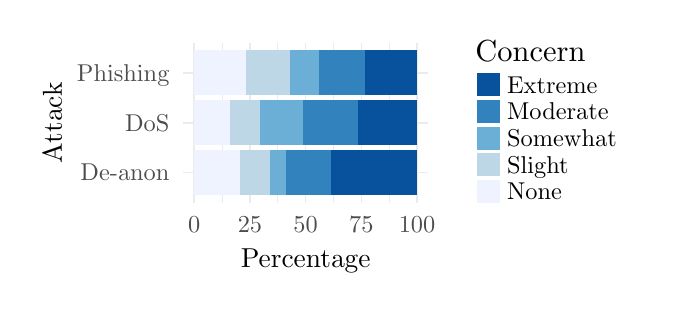
\begin{tikzpicture}[x=1pt,y=1pt]
\definecolor{fillColor}{RGB}{255,255,255}
\path[use as bounding box,fill=fillColor,fill opacity=0.00] (0,0) rectangle (224.04, 93.95);
\begin{scope}
\path[clip] ( 56.18, 30.77) rectangle (144.74, 88.45);
\definecolor{drawColor}{gray}{0.92}

\path[draw=drawColor,line width= 0.3pt,line join=round] ( 70.26, 30.77) --
	( 70.26, 88.45);

\path[draw=drawColor,line width= 0.3pt,line join=round] ( 90.39, 30.77) --
	( 90.39, 88.45);

\path[draw=drawColor,line width= 0.3pt,line join=round] (110.52, 30.77) --
	(110.52, 88.45);

\path[draw=drawColor,line width= 0.3pt,line join=round] (130.64, 30.77) --
	(130.64, 88.45);

\path[draw=drawColor,line width= 0.6pt,line join=round] ( 56.18, 41.59) --
	(144.74, 41.59);

\path[draw=drawColor,line width= 0.6pt,line join=round] ( 56.18, 59.61) --
	(144.74, 59.61);

\path[draw=drawColor,line width= 0.6pt,line join=round] ( 56.18, 77.64) --
	(144.74, 77.64);

\path[draw=drawColor,line width= 0.6pt,line join=round] ( 60.20, 30.77) --
	( 60.20, 88.45);

\path[draw=drawColor,line width= 0.6pt,line join=round] ( 80.33, 30.77) --
	( 80.33, 88.45);

\path[draw=drawColor,line width= 0.6pt,line join=round] (100.45, 30.77) --
	(100.45, 88.45);

\path[draw=drawColor,line width= 0.6pt,line join=round] (120.58, 30.77) --
	(120.58, 88.45);

\path[draw=drawColor,line width= 0.6pt,line join=round] (140.71, 30.77) --
	(140.71, 88.45);
\definecolor{fillColor}{RGB}{239,243,255}

\path[fill=fillColor] ( 60.20, 33.48) rectangle ( 76.78, 49.70);
\definecolor{fillColor}{RGB}{189,215,231}

\path[fill=fillColor] ( 76.78, 33.48) rectangle ( 87.44, 49.70);
\definecolor{fillColor}{RGB}{107,174,214}

\path[fill=fillColor] ( 87.44, 33.48) rectangle ( 93.35, 49.70);
\definecolor{fillColor}{RGB}{49,130,189}

\path[fill=fillColor] ( 93.35, 33.48) rectangle (109.54, 49.70);
\definecolor{fillColor}{RGB}{8,81,156}

\path[fill=fillColor] (109.54, 33.48) rectangle (140.72, 49.70);
\definecolor{fillColor}{RGB}{239,243,255}

\path[fill=fillColor] ( 60.20, 51.50) rectangle ( 73.16, 67.72);
\definecolor{fillColor}{RGB}{189,215,231}

\path[fill=fillColor] ( 73.16, 51.50) rectangle ( 83.77, 67.72);
\definecolor{fillColor}{RGB}{107,174,214}

\path[fill=fillColor] ( 83.77, 51.50) rectangle ( 99.47, 67.72);
\definecolor{fillColor}{RGB}{49,130,189}

\path[fill=fillColor] ( 99.47, 51.50) rectangle (119.50, 67.72);
\definecolor{fillColor}{RGB}{8,81,156}

\path[fill=fillColor] (119.50, 51.50) rectangle (140.71, 67.72);
\definecolor{fillColor}{RGB}{239,243,255}

\path[fill=fillColor] ( 60.20, 69.53) rectangle ( 79.05, 85.75);
\definecolor{fillColor}{RGB}{189,215,231}

\path[fill=fillColor] ( 79.05, 69.53) rectangle ( 94.75, 85.75);
\definecolor{fillColor}{RGB}{107,174,214}

\path[fill=fillColor] ( 94.75, 69.53) rectangle (105.36, 85.75);
\definecolor{fillColor}{RGB}{49,130,189}

\path[fill=fillColor] (105.36, 69.53) rectangle (121.85, 85.75);
\definecolor{fillColor}{RGB}{8,81,156}

\path[fill=fillColor] (121.85, 69.53) rectangle (140.70, 85.75);
\end{scope}
\begin{scope}
\path[clip] (  0.00,  0.00) rectangle (224.04, 93.95);
\definecolor{drawColor}{gray}{0.30}

\node[text=drawColor,anchor=base east,inner sep=0pt, outer sep=0pt, scale=  0.88] at ( 51.23, 38.56) {De-anon};

\node[text=drawColor,anchor=base east,inner sep=0pt, outer sep=0pt, scale=  0.88] at ( 51.23, 56.58) {DoS};

\node[text=drawColor,anchor=base east,inner sep=0pt, outer sep=0pt, scale=  0.88] at ( 51.23, 74.61) {Phishing};
\end{scope}
\begin{scope}
\path[clip] (  0.00,  0.00) rectangle (224.04, 93.95);
\definecolor{drawColor}{gray}{0.30}

\node[text=drawColor,anchor=base,inner sep=0pt, outer sep=0pt, scale=  0.88] at ( 60.20, 19.76) {0};

\node[text=drawColor,anchor=base,inner sep=0pt, outer sep=0pt, scale=  0.88] at ( 80.33, 19.76) {25};

\node[text=drawColor,anchor=base,inner sep=0pt, outer sep=0pt, scale=  0.88] at (100.45, 19.76) {50};

\node[text=drawColor,anchor=base,inner sep=0pt, outer sep=0pt, scale=  0.88] at (120.58, 19.76) {75};

\node[text=drawColor,anchor=base,inner sep=0pt, outer sep=0pt, scale=  0.88] at (140.71, 19.76) {100};
\end{scope}
\begin{scope}
\path[clip] (  0.00,  0.00) rectangle (224.04, 93.95);
\definecolor{drawColor}{RGB}{0,0,0}

\node[text=drawColor,anchor=base,inner sep=0pt, outer sep=0pt, scale=  0.99] at (100.46,  7.44) {Percentage};
\end{scope}
\begin{scope}
\path[clip] (  0.00,  0.00) rectangle (224.04, 93.95);
\definecolor{drawColor}{RGB}{0,0,0}

\node[text=drawColor,rotate= 90.00,anchor=base,inner sep=0pt, outer sep=0pt, scale=  0.99] at ( 12.32, 59.61) {Attack};
\end{scope}
\begin{scope}
\path[clip] (  0.00,  0.00) rectangle (224.04, 93.95);
\definecolor{drawColor}{RGB}{0,0,0}

\node[text=drawColor,anchor=base west,inner sep=0pt, outer sep=0pt, scale=  1.10] at (161.81, 81.72) {Concern};
\end{scope}
\begin{scope}
\path[clip] (  0.00,  0.00) rectangle (224.04, 93.95);
\definecolor{fillColor}{RGB}{8,81,156}

\path[fill=fillColor] (162.52, 69.18) rectangle (170.74, 77.40);
\end{scope}
\begin{scope}
\path[clip] (  0.00,  0.00) rectangle (224.04, 93.95);
\definecolor{fillColor}{RGB}{49,130,189}

\path[fill=fillColor] (162.52, 59.55) rectangle (170.74, 67.76);
\end{scope}
\begin{scope}
\path[clip] (  0.00,  0.00) rectangle (224.04, 93.95);
\definecolor{fillColor}{RGB}{107,174,214}

\path[fill=fillColor] (162.52, 49.91) rectangle (170.74, 58.12);
\end{scope}
\begin{scope}
\path[clip] (  0.00,  0.00) rectangle (224.04, 93.95);
\definecolor{fillColor}{RGB}{189,215,231}

\path[fill=fillColor] (162.52, 40.27) rectangle (170.74, 48.49);
\end{scope}
\begin{scope}
\path[clip] (  0.00,  0.00) rectangle (224.04, 93.95);
\definecolor{fillColor}{RGB}{239,243,255}

\path[fill=fillColor] (162.52, 30.64) rectangle (170.74, 38.85);
\end{scope}
\begin{scope}
\path[clip] (  0.00,  0.00) rectangle (224.04, 93.95);
\definecolor{drawColor}{RGB}{0,0,0}

\node[text=drawColor,anchor=base west,inner sep=0pt, outer sep=0pt, scale=  0.88] at (173.26, 70.26) {Extreme};
\end{scope}
\begin{scope}
\path[clip] (  0.00,  0.00) rectangle (224.04, 93.95);
\definecolor{drawColor}{RGB}{0,0,0}

\node[text=drawColor,anchor=base west,inner sep=0pt, outer sep=0pt, scale=  0.88] at (173.26, 60.62) {Moderate};
\end{scope}
\begin{scope}
\path[clip] (  0.00,  0.00) rectangle (224.04, 93.95);
\definecolor{drawColor}{RGB}{0,0,0}

\node[text=drawColor,anchor=base west,inner sep=0pt, outer sep=0pt, scale=  0.88] at (173.26, 50.99) {Somewhat};
\end{scope}
\begin{scope}
\path[clip] (  0.00,  0.00) rectangle (224.04, 93.95);
\definecolor{drawColor}{RGB}{0,0,0}

\node[text=drawColor,anchor=base west,inner sep=0pt, outer sep=0pt, scale=  0.88] at (173.26, 41.35) {Slight};
\end{scope}
\begin{scope}
\path[clip] (  0.00,  0.00) rectangle (224.04, 93.95);
\definecolor{drawColor}{RGB}{0,0,0}

\node[text=drawColor,anchor=base west,inner sep=0pt, outer sep=0pt, scale=  0.88] at (173.26, 31.71) {None};
\end{scope}
\end{tikzpicture}

    \caption{The level of concern onion service operators have with respect to a
    phishing clone of their service, denial-of-service attacks, and
    deanonymization.}
    \label{fig:onion-operation-concerns}
\end{figure}

\subsubsection{Susceptibility to phishing attacks}

Phishing remains an issue despite onion services' extra anonymity and security
properties.  Past work has uncovered an attack that transparently rewrote
Bitcoin addresses to hijack Bitcoin
transactions~\cite{Winter2016a,Nurmi2015a,Monteiro2016a}.  Key to this attack is
the difficulty of telling apart an authentic from an impersonation domain.  For
conventional domains we rely on (EV) certificates, browser protections, search
results, and long-lived reputation, but none of these methods work well for
onion services.  Does the nature of onion services facilitate phishing attacks?
If so, what can we do to mitigate the issue?

We asked our respondents if they ever thought about the authenticity of an onion
site.  With 80\%, the majority of our respondents did while 20\% didn't.
Clearly, there is a need for verification but how does one verify that an onion
service is authentic?  Figure~\ref{fig:determining-legitimacy} gives an overview
of the strategies that our respondents employ.

\begin{figure}[t]
    \centering
    % Created by tikzDevice version 0.10.1 on 2018-02-09 15:02:27
% !TEX encoding = UTF-8 Unicode
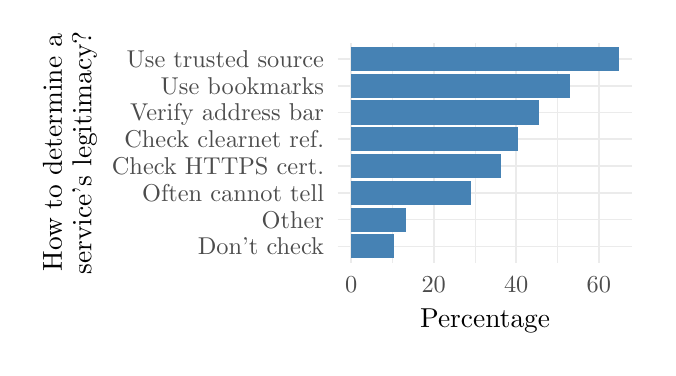
\begin{tikzpicture}[x=1pt,y=1pt]
\definecolor{fillColor}{RGB}{255,255,255}
\path[use as bounding box,fill=fillColor,fill opacity=0.00] (0,0) rectangle (224.04,115.63);
\begin{scope}
\path[clip] (112.04, 30.77) rectangle (218.54,110.13);
\definecolor{drawColor}{gray}{0.92}

\path[draw=drawColor,line width= 0.3pt,line join=round] (131.80, 30.77) --
	(131.80,110.13);

\path[draw=drawColor,line width= 0.3pt,line join=round] (161.62, 30.77) --
	(161.62,110.13);

\path[draw=drawColor,line width= 0.3pt,line join=round] (191.45, 30.77) --
	(191.45,110.13);

\path[draw=drawColor,line width= 0.6pt,line join=round] (112.04, 36.58) --
	(218.54, 36.58);

\path[draw=drawColor,line width= 0.6pt,line join=round] (112.04, 46.26) --
	(218.54, 46.26);

\path[draw=drawColor,line width= 0.6pt,line join=round] (112.04, 55.94) --
	(218.54, 55.94);

\path[draw=drawColor,line width= 0.6pt,line join=round] (112.04, 65.61) --
	(218.54, 65.61);

\path[draw=drawColor,line width= 0.6pt,line join=round] (112.04, 75.29) --
	(218.54, 75.29);

\path[draw=drawColor,line width= 0.6pt,line join=round] (112.04, 84.97) --
	(218.54, 84.97);

\path[draw=drawColor,line width= 0.6pt,line join=round] (112.04, 94.65) --
	(218.54, 94.65);

\path[draw=drawColor,line width= 0.6pt,line join=round] (112.04,104.33) --
	(218.54,104.33);

\path[draw=drawColor,line width= 0.6pt,line join=round] (116.88, 30.77) --
	(116.88,110.13);

\path[draw=drawColor,line width= 0.6pt,line join=round] (146.71, 30.77) --
	(146.71,110.13);

\path[draw=drawColor,line width= 0.6pt,line join=round] (176.53, 30.77) --
	(176.53,110.13);

\path[draw=drawColor,line width= 0.6pt,line join=round] (206.36, 30.77) --
	(206.36,110.13);
\definecolor{fillColor}{RGB}{70,130,180}

\path[fill=fillColor] (116.88, 32.22) rectangle (132.50, 40.93);

\path[fill=fillColor] (116.88, 41.90) rectangle (136.54, 50.61);

\path[fill=fillColor] (116.88, 51.58) rectangle (160.24, 60.29);

\path[fill=fillColor] (116.88, 61.26) rectangle (171.21, 69.97);

\path[fill=fillColor] (116.88, 70.94) rectangle (177.28, 79.65);

\path[fill=fillColor] (116.88, 80.61) rectangle (184.80, 89.32);

\path[fill=fillColor] (116.88, 90.29) rectangle (195.79, 99.00);

\path[fill=fillColor] (116.88, 99.97) rectangle (213.70,108.68);
\end{scope}
\begin{scope}
\path[clip] (  0.00,  0.00) rectangle (224.04,115.63);
\definecolor{drawColor}{gray}{0.30}

\node[text=drawColor,anchor=base east,inner sep=0pt, outer sep=0pt, scale=  0.88] at (107.09, 33.55) {Don't check};

\node[text=drawColor,anchor=base east,inner sep=0pt, outer sep=0pt, scale=  0.88] at (107.09, 43.23) {Other};

\node[text=drawColor,anchor=base east,inner sep=0pt, outer sep=0pt, scale=  0.88] at (107.09, 52.91) {Often cannot tell};

\node[text=drawColor,anchor=base east,inner sep=0pt, outer sep=0pt, scale=  0.88] at (107.09, 62.58) {Check HTTPS cert.};

\node[text=drawColor,anchor=base east,inner sep=0pt, outer sep=0pt, scale=  0.88] at (107.09, 72.26) {Check clearnet ref.};

\node[text=drawColor,anchor=base east,inner sep=0pt, outer sep=0pt, scale=  0.88] at (107.09, 81.94) {Verify address bar};

\node[text=drawColor,anchor=base east,inner sep=0pt, outer sep=0pt, scale=  0.88] at (107.09, 91.62) {Use bookmarks};

\node[text=drawColor,anchor=base east,inner sep=0pt, outer sep=0pt, scale=  0.88] at (107.09,101.29) {Use trusted source};
\end{scope}
\begin{scope}
\path[clip] (  0.00,  0.00) rectangle (224.04,115.63);
\definecolor{drawColor}{gray}{0.30}

\node[text=drawColor,anchor=base,inner sep=0pt, outer sep=0pt, scale=  0.88] at (116.88, 19.76) {0};

\node[text=drawColor,anchor=base,inner sep=0pt, outer sep=0pt, scale=  0.88] at (146.71, 19.76) {20};

\node[text=drawColor,anchor=base,inner sep=0pt, outer sep=0pt, scale=  0.88] at (176.53, 19.76) {40};

\node[text=drawColor,anchor=base,inner sep=0pt, outer sep=0pt, scale=  0.88] at (206.36, 19.76) {60};
\end{scope}
\begin{scope}
\path[clip] (  0.00,  0.00) rectangle (224.04,115.63);
\definecolor{drawColor}{RGB}{0,0,0}

\node[text=drawColor,anchor=base,inner sep=0pt, outer sep=0pt, scale=  0.99] at (165.29,  7.44) {Percentage};
\end{scope}
\begin{scope}
\path[clip] (  0.00,  0.00) rectangle (224.04,115.63);
\definecolor{drawColor}{RGB}{0,0,0}

\node[text=drawColor,rotate= 90.00,anchor=base,inner sep=0pt, outer sep=0pt, scale=  0.99] at ( 12.32, 70.45) {How to determine a};

\node[text=drawColor,rotate= 90.00,anchor=base,inner sep=0pt, outer sep=0pt, scale=  0.99] at ( 23.01, 70.45) {service's legitimacy?};
\end{scope}
\end{tikzpicture}

    \caption{How our respondents determine an onion service's legitimacy.}
    \label{fig:determining-legitimacy}
\end{figure}

More than half either consult trusted sources (\eg friends or another web site)
or use bookmarks when revisiting onion services.  Many respondents also verify
the domain in the browser's address bar (46\%), check if the corresponding web
site has a link to its onion site (41\%), or hope that the onion service has an
HTTPS certificate (36\%).\footnote{DigiCert is issuing EV-certificates for onion
sites~\cite{DigiCert2015a} but adoption has been slow---presumably in part
because EV certificates require the CA to verify the applicant's identity
and they are not for free.}  Alarmingly, almost 30\% of respondents stated that
they sometimes cannot tell the difference between an authentic service and an
impersonation, and 11\% never check a service's legitimacy in the first place.
People who selected ``Other'' provided a wide variety of ad-hoc phishing
protections---some clearly misguided, which reinforces the scope of the problem.

Originally meant to improve usability, vanity onion domains also play a role in
the context of phishing.  There is concern that the short and recognizable
prefixes tempt users to only verify the prefix and ignore subsequent
characters~\cite{Winter2015a}.  This oversight may allow attackers to create
impersonation domains that feature the prefix but differ in subsequent
characters.  Nurmi~\cite{Nurmi2015a} and Monteiro~\cite{Monteiro2016a} have both
documented such an attack but its effectiveness is not known.

The majority of our respondents appreciates vanity domains because they are easy
to remember (64\%), easy to recognize (64\%), and they provide a unique
``branding'' (34\%).  Some responses indicate that a vanity prefix conveniently
informs about an onion service's topic, letting visitors know what to expect.
Only 8\% dislike vanity onion domains and 15\% don't have an opinion.
Interestingly, some respondents consider vanity domains unfair because wealthy
entities can afford to generate longer prefixes.  Several respondents voiced
their concern that vanity domains create a false sense of security and
facilitate phishing attacks.  In a separate question we inquired how many
characters our respondents verify in onion domains.  43\% verify 13--16 digits,
\ie (almost) the full domain, while 46\% verify up to nine digits, which is
within the realm of brute force attacks.  Finally, a handful number of
respondents cited misguided reasons why they dislike vanity domains, \eg some
believe that vanity domains are a sign of weak hash functions while others
believe that vanity domains make the onion service ``less hidden'' or allow
somebody to create ``the same private key.''

\subsubsection{Perceived security}

Questions 6.4 and 6.6 asked how safe our respondents feel when using Tor Browser
and onion services, respectively.  Figure~\ref{fig:perceived-security} shows the
results.  Using Tor Browser makes 86\% of our respondents feel at least somewhat
safe.  The same is true for 67\% when using onion services---clearly not as many
as for Tor Browser.

\begin{figure}[t]
    \centering
    % Created by tikzDevice version 0.10.1 on 2018-02-09 14:21:58
% !TEX encoding = UTF-8 Unicode
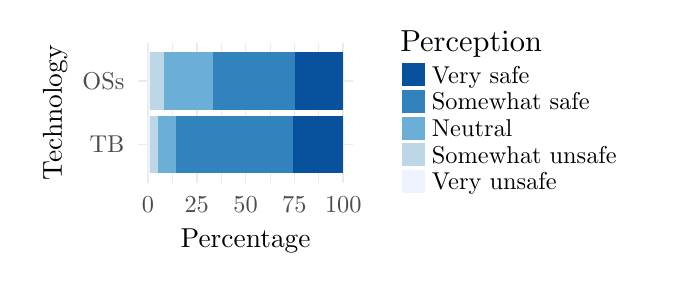
\begin{tikzpicture}[x=1pt,y=1pt]
\definecolor{fillColor}{RGB}{255,255,255}
\path[use as bounding box,fill=fillColor,fill opacity=0.00] (0,0) rectangle (224.04, 86.72);
\begin{scope}
\path[clip] ( 39.91, 30.77) rectangle (117.57, 81.22);
\definecolor{drawColor}{gray}{0.92}

\path[draw=drawColor,line width= 0.3pt,line join=round] ( 52.27, 30.77) --
	( 52.27, 81.22);

\path[draw=drawColor,line width= 0.3pt,line join=round] ( 69.92, 30.77) --
	( 69.92, 81.22);

\path[draw=drawColor,line width= 0.3pt,line join=round] ( 87.56, 30.77) --
	( 87.56, 81.22);

\path[draw=drawColor,line width= 0.3pt,line join=round] (105.21, 30.77) --
	(105.21, 81.22);

\path[draw=drawColor,line width= 0.6pt,line join=round] ( 39.91, 44.53) --
	(117.57, 44.53);

\path[draw=drawColor,line width= 0.6pt,line join=round] ( 39.91, 67.46) --
	(117.57, 67.46);

\path[draw=drawColor,line width= 0.6pt,line join=round] ( 43.44, 30.77) --
	( 43.44, 81.22);

\path[draw=drawColor,line width= 0.6pt,line join=round] ( 61.09, 30.77) --
	( 61.09, 81.22);

\path[draw=drawColor,line width= 0.6pt,line join=round] ( 78.74, 30.77) --
	( 78.74, 81.22);

\path[draw=drawColor,line width= 0.6pt,line join=round] ( 96.39, 30.77) --
	( 96.39, 81.22);

\path[draw=drawColor,line width= 0.6pt,line join=round] (114.04, 30.77) --
	(114.04, 81.22);
\definecolor{fillColor}{RGB}{239,243,255}

\path[fill=fillColor] ( 43.44, 34.21) rectangle ( 44.12, 54.85);
\definecolor{fillColor}{RGB}{189,215,231}

\path[fill=fillColor] ( 44.12, 34.21) rectangle ( 47.24, 54.85);
\definecolor{fillColor}{RGB}{107,174,214}

\path[fill=fillColor] ( 47.24, 34.21) rectangle ( 53.62, 54.85);
\definecolor{fillColor}{RGB}{49,130,189}

\path[fill=fillColor] ( 53.62, 34.21) rectangle ( 95.71, 54.85);
\definecolor{fillColor}{RGB}{8,81,156}

\path[fill=fillColor] ( 95.71, 34.21) rectangle (114.04, 54.85);
\definecolor{fillColor}{RGB}{239,243,255}

\path[fill=fillColor] ( 43.44, 57.15) rectangle ( 44.26, 77.78);
\definecolor{fillColor}{RGB}{189,215,231}

\path[fill=fillColor] ( 44.26, 57.15) rectangle ( 49.32, 77.78);
\definecolor{fillColor}{RGB}{107,174,214}

\path[fill=fillColor] ( 49.32, 57.15) rectangle ( 67.07, 77.78);
\definecolor{fillColor}{RGB}{49,130,189}

\path[fill=fillColor] ( 67.07, 57.15) rectangle ( 96.70, 77.78);
\definecolor{fillColor}{RGB}{8,81,156}

\path[fill=fillColor] ( 96.70, 57.15) rectangle (114.04, 77.78);
\end{scope}
\begin{scope}
\path[clip] (  0.00,  0.00) rectangle (224.04, 86.72);
\definecolor{drawColor}{gray}{0.30}

\node[text=drawColor,anchor=base east,inner sep=0pt, outer sep=0pt, scale=  0.88] at ( 34.96, 41.50) {TB};

\node[text=drawColor,anchor=base east,inner sep=0pt, outer sep=0pt, scale=  0.88] at ( 34.96, 64.43) {OSs};
\end{scope}
\begin{scope}
\path[clip] (  0.00,  0.00) rectangle (224.04, 86.72);
\definecolor{drawColor}{gray}{0.30}

\node[text=drawColor,anchor=base,inner sep=0pt, outer sep=0pt, scale=  0.88] at ( 43.44, 19.76) {0};

\node[text=drawColor,anchor=base,inner sep=0pt, outer sep=0pt, scale=  0.88] at ( 61.09, 19.76) {25};

\node[text=drawColor,anchor=base,inner sep=0pt, outer sep=0pt, scale=  0.88] at ( 78.74, 19.76) {50};

\node[text=drawColor,anchor=base,inner sep=0pt, outer sep=0pt, scale=  0.88] at ( 96.39, 19.76) {75};

\node[text=drawColor,anchor=base,inner sep=0pt, outer sep=0pt, scale=  0.88] at (114.04, 19.76) {100};
\end{scope}
\begin{scope}
\path[clip] (  0.00,  0.00) rectangle (224.04, 86.72);
\definecolor{drawColor}{RGB}{0,0,0}

\node[text=drawColor,anchor=base,inner sep=0pt, outer sep=0pt, scale=  0.99] at ( 78.74,  7.44) {Percentage};
\end{scope}
\begin{scope}
\path[clip] (  0.00,  0.00) rectangle (224.04, 86.72);
\definecolor{drawColor}{RGB}{0,0,0}

\node[text=drawColor,rotate= 90.00,anchor=base,inner sep=0pt, outer sep=0pt, scale=  0.99] at ( 12.32, 56.00) {Technology};
\end{scope}
\begin{scope}
\path[clip] (  0.00,  0.00) rectangle (224.04, 86.72);
\definecolor{drawColor}{RGB}{0,0,0}

\node[text=drawColor,anchor=base west,inner sep=0pt, outer sep=0pt, scale=  1.10] at (134.64, 78.11) {Perception};
\end{scope}
\begin{scope}
\path[clip] (  0.00,  0.00) rectangle (224.04, 86.72);
\definecolor{fillColor}{RGB}{8,81,156}

\path[fill=fillColor] (135.35, 65.57) rectangle (143.56, 73.78);
\end{scope}
\begin{scope}
\path[clip] (  0.00,  0.00) rectangle (224.04, 86.72);
\definecolor{fillColor}{RGB}{49,130,189}

\path[fill=fillColor] (135.35, 55.93) rectangle (143.56, 64.15);
\end{scope}
\begin{scope}
\path[clip] (  0.00,  0.00) rectangle (224.04, 86.72);
\definecolor{fillColor}{RGB}{107,174,214}

\path[fill=fillColor] (135.35, 46.30) rectangle (143.56, 54.51);
\end{scope}
\begin{scope}
\path[clip] (  0.00,  0.00) rectangle (224.04, 86.72);
\definecolor{fillColor}{RGB}{189,215,231}

\path[fill=fillColor] (135.35, 36.66) rectangle (143.56, 44.87);
\end{scope}
\begin{scope}
\path[clip] (  0.00,  0.00) rectangle (224.04, 86.72);
\definecolor{fillColor}{RGB}{239,243,255}

\path[fill=fillColor] (135.35, 27.03) rectangle (143.56, 35.24);
\end{scope}
\begin{scope}
\path[clip] (  0.00,  0.00) rectangle (224.04, 86.72);
\definecolor{drawColor}{RGB}{0,0,0}

\node[text=drawColor,anchor=base west,inner sep=0pt, outer sep=0pt, scale=  0.88] at (146.08, 66.65) {Very safe};
\end{scope}
\begin{scope}
\path[clip] (  0.00,  0.00) rectangle (224.04, 86.72);
\definecolor{drawColor}{RGB}{0,0,0}

\node[text=drawColor,anchor=base west,inner sep=0pt, outer sep=0pt, scale=  0.88] at (146.08, 57.01) {Somewhat safe};
\end{scope}
\begin{scope}
\path[clip] (  0.00,  0.00) rectangle (224.04, 86.72);
\definecolor{drawColor}{RGB}{0,0,0}

\node[text=drawColor,anchor=base west,inner sep=0pt, outer sep=0pt, scale=  0.88] at (146.08, 47.37) {Neutral};
\end{scope}
\begin{scope}
\path[clip] (  0.00,  0.00) rectangle (224.04, 86.72);
\definecolor{drawColor}{RGB}{0,0,0}

\node[text=drawColor,anchor=base west,inner sep=0pt, outer sep=0pt, scale=  0.88] at (146.08, 37.74) {Somewhat unsafe};
\end{scope}
\begin{scope}
\path[clip] (  0.00,  0.00) rectangle (224.04, 86.72);
\definecolor{drawColor}{RGB}{0,0,0}

\node[text=drawColor,anchor=base west,inner sep=0pt, outer sep=0pt, scale=  0.88] at (146.08, 28.10) {Very unsafe};
\end{scope}
\end{tikzpicture}

    \caption{The level of security our respondents perceive when using Tor
    Browser (TB) and onion services (OSs).}
    \label{fig:perceived-security}
\end{figure}

Asked about why our respondents feel that way about Tor Browser, our results
reveal that non-experts lack the ability to evaluate (or even understand) Tor's
design which is why they defer to expert opinion, their gut feeling, or the
trust they have in Tor developers.  The Tor Project is perceived to take
security and privacy more seriously than any other browser vendor, which is
appreciated among our respondents.  Most of our respondents' criticism focused
not on Tor Browser but on the underlying Firefox code base.  Many participants
were unhappy with the exploit mitigation techniques, the lack of sandboxing, and
the complex code base.  Chrome was sometimes brought up as the golden standard
for browser security.\footnote{Note that our survey was run before Mozilla
released Firefox Quantum on Nov 14, 2017, which brought substantial improvements
in both security and usability.}  Malicious exit relays were a concern for a
handful of participants while another couple of participants are concerned that
their use of Tor makes them stick out and turn into a target for government
agencies.  Some participants weren't sure if their Tor setup works properly---a
common theme that we also noticed in our interviews: Non-technical users desire
visual feedback confirming that their network traffic comes out ``somewhere
else.''

With respect to onion services, the majority expressed that the added security
and anonymity makes them feel safe.  Another factor contributing to the
perceived security is that onion services make use of far fewer advertising
companies.  Orthogonal to the technology, many participants voiced concern about
illegal and questionable content on onion services, described by some as a
``Wild West.''  Phishing sites, honeypots, and compromised onion sites further
contribute to this perception.


\section{Discussion}
\label{sec:discussion}

\subsection{Biases}

It is difficult to draw a truly uniform sample of Tor users.  The only way to
reach all Tor users uniformly would be to modify Tor Browser's landing page
that is displayed on start---an approach that we considered prohibitively
invasive.  Instead, we decided to ask The Tor Project to disseminate our survey
on its blog and social media accounts.  We believe that this recruitment
strategy was subject to the following biases.

\paragraph{Non-response bias.} 
People who noticed our call for volunteers and decided against participating
may exhibit traits that are fundamentally different from those who did
participate.  These non-respondents may have valued their privacy too much,
falsely believed that their experience is irrelevant, lacked the time, or had
other reasons not to participate.

\paragraph{Survivor bias.}
We predominantly heard from people who can tolerate Tor's usability issues,
which is why they are still around to tell their tale.  We likely did not hear
from many---if any---people who gave up on Tor and were thus unable to tell us
what drove them away.  The danger of survivor bias lies in optimizing the user
experience for the subset of people who can tolerate a non-optimal user
experience.

\paragraph{Self-selection bias.}
Due to the nature of our online survey, participants could voluntarily select
themselves into the group of respondents.  This set of people may be unusually
engaged and technical, which is why they have formed opinions that they
consider worth sharing.

\subsection{Take-aways for Tor developers}

Several of our interview participants pointed out Tor Browser's antiquated user
interface.  Past work has shown that users interpret unrelated aspects such as
voice quality as a proxy signal for security, which raises the question if the
same holds true for user interface design~\cite[\S~IV.A]{Abu-Salma2017a}.  If
so, it is important to equip Tor Browser with a modern user interface.

\begin{figure}[t]
    \centering
    \includegraphics[width=\linewidth]{figures/tor-comic.jpg}
    \caption{A comic draft that illustrates what Tor can and cannot provide for
        non-technical users.  The comic was drawn by artist Jason Li while
        working with one of the authors.}
    \label{fig:tor-comic}
\end{figure}

\subsection{Take-aways for Tor users}

The strong security properties of onion services are futile if users cannot tell
apart a genuine domain from its impersonation.  Awareness of this issue is the
first step and several onion services have long begun to alert their users.



% could tor show you when an onion service descriptor was first published?


\subsection{Take-aways for Tor researchers}

We found it challenging, yet rewarding and illuminating to study the Tor
community.  Tor users obviously value their privacy which reduces their
willingness to participate in research projects.  Past academic research
projects that involved questionable methods turned this care into distrust for
many users.  Showing willingness to directly interact with the community and
taking seriously their concerns signals respect and transparent methods.  For
our online survey, we recommend to use software that works in Tor
Browser\footnote{Note that Tor Browser supports three security levels; the
default of ``low,'' ``medium,'' and ``high.''  Some users brought to our
attention that our survey did not work when the security level is set to
``high'' because it disables JavaScript, which our survey required---an
oversight on our end.} and does not fetch tracking scripts such as Google
Analytics.  For the survey design, one likely has to forego asking questions
that are best practice such as income level and country of residence.  We made
even the basic information we asked optional so our respondents had the chance
to answer the survey without providing any personal information at all.  In our
interviews we tried to accomodate the needs of our participants by using
software of their choice.


\section{Conclusion}
\label{sec:conclusion}

In this work we studied how Tor users interact with onion services and the
broader technology that enables onion services.  Drawing on a mixed-methods
approach, we conducted seventeen semi-structured interviews and collected 828
responses to our online survey.  These two data sets served as the basis of our
analysis and provided unique insight into how Tor users perceive, use, and
understand Tor in general and onion services in particular.

We find that the current state of onion services resembles the web of the 90s.
Pages load slowly, user interfaces are clumsy, and search engines fall short of
expectations.  Users appreciate the extra security, privacy, and \textsc{nat}
punching properties of onion services, giving rise to numerous use cases, but
are frequently wary of the content that is hosted on them.  Some users found
ways to manage what is perhaps the most striking idiosyncracy of onion
services---their domain format---by using bookmarks, (encrypted) files
containing links, and referring to trusted link aggregators.  Many users however
have flawed mental models of onion services that could increase their
susceptibility to phishing attacks.

Our code, data, and auxiliary resources are available on our project page at
\url{https://nymity.ch/onion-services/}.


\section*{Acknowledgements}
We want to thank George Kadianakis for helpful feedback.

We want to thank Laura M. Roberts, Roya Ensafi, Will Scott, and Jens Kubiziel
for help with pre-testing the survey.

Thanks to Katherine Haenschen for helping us improve our method.

This research was supported in part by the Center for Information Technology
Policy at Princeton University.  This project was further supported in part by
National Science Foundation Awards CNS-1540055 and CNS-1602399.


\balance

{\footnotesize
\printbibliography}

\end{document}
